% !TEX program = xelatex
\documentclass[10pt, aspectratio=169]{beamer}

\usepackage{fontspec}
\setmainfont{Times New Roman}
\setsansfont{Calibri}

\usepackage{graphicx}
\usepackage{booktabs}
\usepackage{tabularx}
\usepackage{colortbl}
\usepackage{tikz}
\usepackage{multicol}
\usepackage{caption}
\usepackage{multirow}
\usepackage{array}
\usepackage{amsmath}
\usepackage{amssymb}
\usepackage{xcolor}
\usepackage{appendixnumberbeamer}

% =====================  Theme USTH Blue  =====================
\definecolor{usthblue}{RGB}{0, 84, 166}
\definecolor{usthlight}{RGB}{220, 232, 247}
\definecolor{usthred}{RGB}{237, 28, 36}
\definecolor{usthaccent}{RGB}{0, 132, 209}
\definecolor{usthdark}{RGB}{0, 51, 102}
\definecolor{softgray}{RGB}{245, 245, 245}
\definecolor{goodgreen}{RGB}{34, 139, 34}

\usetheme{Madrid}
\usecolortheme[named=usthblue]{structure}
\setbeamercolor{title}{fg=white,bg=usthblue}
\setbeamercolor{frametitle}{fg=white,bg=usthblue}
\setbeamercolor{block title}{fg=white,bg=usthaccent}
\setbeamercolor{block body}{bg=usthlight!40}
\setbeamercolor{item}{fg=usthblue}
\setbeamercolor{section in toc}{fg=usthdark}
\setbeamertemplate{navigation symbols}{}
\setbeamertemplate{blocks}[rounded][shadow=true]
\setbeamertemplate{itemize item}{\color{usthblue}$\blacktriangleright$}
\setbeamertemplate{itemize subitem}{\color{usthaccent}$\bullet$}

% Framesubtitle rendered in the white body, just below the blue header, left-aligned
\makeatletter
\renewcommand{\framesubtitle}[1]{%
  \vspace*{-0.3em}\noindent{\large\bfseries\textcolor{usthdark}{#1}}\par\vspace{0.6em}%
}
\makeatother

\setbeamertemplate{footline}{%
  \leavevmode%
  \hbox{%
    \begin{beamercolorbox}[wd=.32\paperwidth,ht=2.4ex,dp=1ex,left]{author in head/foot}%
      \hspace*{2ex}\insertshortauthor
    \end{beamercolorbox}%
    \begin{beamercolorbox}[wd=.45\paperwidth,ht=2.4ex,dp=1ex,center]{title in head/foot}%
      \insertshorttitle
    \end{beamercolorbox}%
    \begin{beamercolorbox}[wd=.23\paperwidth,ht=2.4ex,dp=1ex,right]{date in head/foot}%
      \insertframenumber{} / \inserttotalframenumber\hspace*{2ex}
    \end{beamercolorbox}}%
}

% =====================  Title info  =====================
\title[Skin Lesion Classification with Deep Learning]{\large A Comparative Evaluation of Deep Learning Models \\ for Skin Lesion Classification on Dermoscopic Images}
\subtitle{\small An Ensemble and Interpretability Approach using Grad-CAM}
\author[Nguyen Trong Bach]{Nguyen Trong Bach \textemdash{} 23BI14057 \\[2pt]
\footnotesize \textbf{Internal Supervisor:} Dr.\ Nghiem Thi Phuong \quad \textbf{External Supervisor:} Dr.\ Vu Trong Sinh}
\institute[USTH]{\footnotesize Department of Information and Communication Technology \\ University of Science and Technology of Hanoi}
\date{\footnotesize July 2026}

\titlegraphic{
\includegraphics[height=1.3cm]{../thesis/figures/logo.png}}

\begin{document}

% =====================  Title page  =====================
\begin{frame}[plain]
    \titlepage
\end{frame}

% =====================  Outline  =====================
\begin{frame}{Outline}
    \begin{columns}
        \column{0.55\textwidth}
        \tableofcontents[hideallsubsections]
        \column{0.45\textwidth}
        \begin{block}{Focus of the thesis}
            \footnotesize
            Build and evaluate a complete deep learning pipeline for 7-class skin lesion classification on ISIC 2018, combining \textbf{four architectures} via \textbf{soft-voting ensemble} and explaining decisions through \textbf{Grad-CAM}.
        \end{block}
    \end{columns}
\end{frame}

% =========================================================
\section{Introduction}
% =========================================================
\begin{frame}{Introduction}
    \framesubtitle{Problem \& Objectives}
    \begin{block}{The clinical problem}
        \small
        Melanoma is the deadliest form of skin cancer --- yet when caught early, more than \textbf{99\%} of patients live past five years. Dermoscopy lets doctors look at a lesion up close, but the final call still depends on how experienced the dermatologist is.
    \end{block}
    \vspace{0.15cm}
    \begin{columns}[T]
        \column{0.5\textwidth}
        \textbf{Three barriers:}
        \begin{itemize}\footnotesize
            \item \textbf{Data imbalance} --- the majority class overwhelms rare cancers.
            \item \textbf{Morphological similarity} --- melanoma and nevi are easily confused.
            \item \textbf{Black-box behaviour} --- doctors cannot trust an unexplained decision.
        \end{itemize}

        \column{0.5\textwidth}
        \textbf{Four contributions:}
        \begin{enumerate}\footnotesize
            \item Imbalance-aware training pipeline.
            \item Fair comparison of 3 CNNs + 1 Transformer.
            \item Soft-voting ensemble that beats every single model.
            \item Grad-CAM + Streamlit demo for clinical trust.
        \end{enumerate}
    \end{columns}
\end{frame}

% =========================================================
\section{Data and Challenges}
% =========================================================
\begin{frame}{Data and Challenges}
    \framesubtitle{ISIC 2018 Task 3 (HAM10000) --- 10,015 dermoscopy images, 7 classes}
    \begin{columns}[T]
        \column{0.5\textwidth}
        \scriptsize
        \begin{table}[]
            \centering
            \begin{tabular}{lrrrr}
            \toprule
            \rowcolor{usthblue!25} \textbf{Class} & \textbf{Train} & \textbf{Val} & \textbf{Test} & \textbf{\%} \\
            \midrule
            NV (Nevus)          & 4\,693 & 1\,006 & 1\,006 & 66.9 \\
            MEL (Melanoma)      &   779  &  167   &  167   & 11.1 \\
            BKL (Benign Ker.)   &   769  &  165   &  165   & 11.0 \\
            BCC (Basal Cell)    &   360  &   77   &   77   &  5.1 \\
            AKIEC (Actinic)     &   229  &   49   &   49   &  3.3 \\
            VASC (Vascular)     &    99  &   21   &   22   &  1.4 \\
            DF (Dermatofibroma) &    81  &   17   &   17   &  1.1 \\
            \midrule
            \textbf{Total}      & \textbf{7\,010} & \textbf{1\,502} & \textbf{1\,503} & 100 \\
            \bottomrule
            \end{tabular}
        \end{table}
        \vspace{0.1cm}
        \centering
        \textcolor{usthred}{\footnotesize Extreme imbalance: \textbf{NV : DF $\approx$ 58 : 1}}

        \column{0.5\textwidth}
        \begin{block}{Why this matters}
            \footnotesize
            Predicting "NV for everything" already yields $\sim$67\% Accuracy --- clinically useless. We optimise \textbf{Macro F1} and \textbf{Macro AUC} instead, so every class counts equally.
        \end{block}
        \vspace{0.2cm}
        \begin{block}{Four counter-mechanisms}
            \footnotesize
            \begin{enumerate}
                \item \textbf{Weighted Sampler} --- balances mini-batches.
                \item \textbf{Mixup / CutMix} --- smooths boundaries.
                \item \textbf{Label Smoothing} --- reduces over-confidence.
                \item \textbf{Macro F1} for checkpoint selection.
            \end{enumerate}
        \end{block}
    \end{columns}
\end{frame}

% =========================================================
\section{Methodology}
% =========================================================
\begin{frame}{Methodology}
    \framesubtitle{Pipeline Overview}
    \vspace{0.1cm}
    \begin{center}
        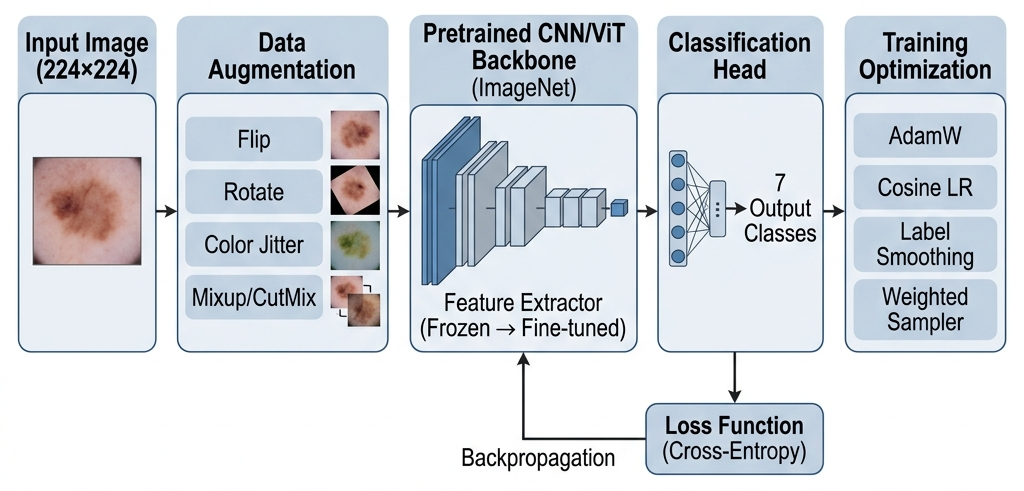
\includegraphics[width=0.88\textwidth,height=0.72\textheight,keepaspectratio]{../thesis/figures/training_pipeline_cropped.png}
    \end{center}
    \vspace{0.15cm}
    {\centering \scriptsize \textit{End-to-end pipeline: preprocessing, augmentation, weighted sampler, Mixup/CutMix, fine-tuning from pretrained weights, evaluation on the test set.}\par}
\end{frame}

\begin{frame}{Methodology}
    \framesubtitle{The Four Architectures Compared}
    \scriptsize
    \begin{table}[]
        \centering
        \begin{tabular}{lcll}
        \toprule
        \rowcolor{usthblue!25}
        \textbf{Model} & \textbf{Params} & \textbf{Design principle} & \textbf{Role in the ensemble} \\
        \midrule
        EfficientNet-B0 & 5.3M  & MBConv $+$ SE, compound scaling           & Compact CNN, fine local features \\
        ResNet50        & 25.6M & Bottleneck residual                       & Deep CNN, classical baseline     \\
        DenseNet121     & 8.0M  & Dense connectivity, feature reuse         & CNN exploiting feature reuse     \\
        Swin-Tiny       & 28.0M & Shifted-window self-attention             & Vision Transformer, global context \\
        \bottomrule
        \end{tabular}
    \end{table}

    \vspace{0.3cm}
    \footnotesize
    \begin{itemize}
        \item All models are \textbf{fine-tuned from ImageNet pretrained weights} through the \texttt{timm} library.
        \item The output head is replaced by \texttt{Linear($d$, 7)}, with dropout 0.25--0.30 before the classifier.
        \item The four diverse backbones allow the ensemble to exploit \textbf{uncorrelated errors} between CNNs and the Transformer.
    \end{itemize}
\end{frame}

\begin{frame}{Methodology}
    \framesubtitle{Training Strategy}
    \begin{columns}[T]
        \column{0.5\textwidth}
        \begin{block}{Mixup \& CutMix\ \footnotesize($p = 0.5$ each)}
            \scriptsize
            \textbf{Mixup:} $\tilde{x} = \lambda x_i + (1-\lambda) x_j$ with $\lambda \sim \mathrm{Beta}(0.2, 0.2)$.\\[2pt]
            \textbf{CutMix:} paste a random patch between two images, the mixed label follows the area ratio.\\[3pt]
            $\Rightarrow$ prevents memorising rare samples and smooths decision boundaries.
        \end{block}

        \begin{block}{Label Smoothing\ \footnotesize($\varepsilon = 0.1$)}
            \scriptsize
            $y_{\text{smooth}} = (1-\varepsilon) \cdot y_{\text{onehot}} + \varepsilon / C$\\[2pt]
            $\Rightarrow$ reduces over-confidence, improves calibration.
        \end{block}

        \column{0.5\textwidth}
        \begin{block}{Weighted Random Sampler}
            \scriptsize
            Per-sample weight: $w_c = \dfrac{N}{C \cdot n_c}$\\[2pt]
            Each batch is approximately balanced across the 7 classes \textemdash{} boosting exposure to DF/VASC.
        \end{block}

        \begin{block}{Optimisation setup}
            \scriptsize
            \textbf{Optimizer:} AdamW, cosine annealing $+$ linear warmup.\\
            \textbf{Mixed precision:} FP16 (about $-40\%$ GPU memory).\\
            \textbf{Gradient clipping:} $\|\nabla\|_{\max} = 1.0$.\\
            \textbf{Early stopping:} patience $= 12$ epochs on Macro F1.
        \end{block}
    \end{columns}
    \vspace{0.15cm}
    {\centering \scriptsize \textit{Per-backbone hyperparameters (learning rate, weight decay, warmup): see appendix A24.}\par}
\end{frame}

% =========================================================
\section{Experimental Results}
% =========================================================
\begin{frame}{Experimental Results}
    \framesubtitle{Single Models and the Ensemble}
    \scriptsize
    \begin{table}[]
        \centering
        \begin{tabular}{lcccc}
        \toprule
        \rowcolor{usthblue!25}
        \textbf{Model} & \textbf{Params} & \textbf{Accuracy} & \textbf{Macro F1} & \textbf{Macro AUC} \\
        \midrule
        EfficientNet-B0 & 5.3M  & 0.8836 & 0.8311 & 0.9522 \\
        ResNet50        & 25.6M & 0.8603 & 0.7902 & 0.9565 \\
        DenseNet121     & 8.0M  & 0.8543 & 0.7967 & 0.9587 \\
        Swin-Tiny       & 28.0M & 0.8490 & 0.7855 & 0.9600 \\
        \rowcolor{usthlight} \textbf{Ensemble (soft-voting)} & --- & \textbf{0.8949} & \textbf{0.8450} & \textbf{0.9803} \\
        \bottomrule
        \end{tabular}
    \end{table}

    \vspace{0.3cm}
    \begin{columns}[T]
        \column{0.55\textwidth}
        \begin{block}{Robustness --- 5 random seeds}
            \footnotesize
            Ensemble Acc \textbf{89.93 $\pm$ 0.66\%}, F1 \textbf{0.852 $\pm$ 0.010}, AUC \textbf{0.982 $\pm$ 0.001}. \\[2pt]
            McNemar's test: ensemble beats every single backbone with $p < 10^{-7}$ vs.\ strongest, $p < 10^{-38}$ vs.\ weakest.
        \end{block}

        \column{0.45\textwidth}
        \begin{block}{Why soft voting works}
            \footnotesize
            CNNs catch local textures, Swin catches global structure. Averaging four uncorrelated probability vectors reduces variance --- no extra training, four inference passes.
        \end{block}
    \end{columns}
\end{frame}

\begin{frame}{Experimental Results}
    \framesubtitle{Ensemble Confusion Matrix}
    \begin{columns}[T]
        \column{0.42\textwidth}
        \footnotesize
        
        \begin{itemize}
            \item A high diagonal $\Rightarrow$ strong recall across every class.
            \item \textbf{DF and VASC} are rare yet still recognised accurately --- thanks to Mixup $+$ the Weighted Sampler.
            \item Residual confusion is concentrated in the \textbf{MEL $\leftrightarrow$ NV $\leftrightarrow$ BKL} cluster, which shares morphology.
            \item No class "disappears" --- the typical failure mode of imbalanced data is avoided.
        \end{itemize}

        \column{0.58\textwidth}
        \begin{figure}
            \centering
            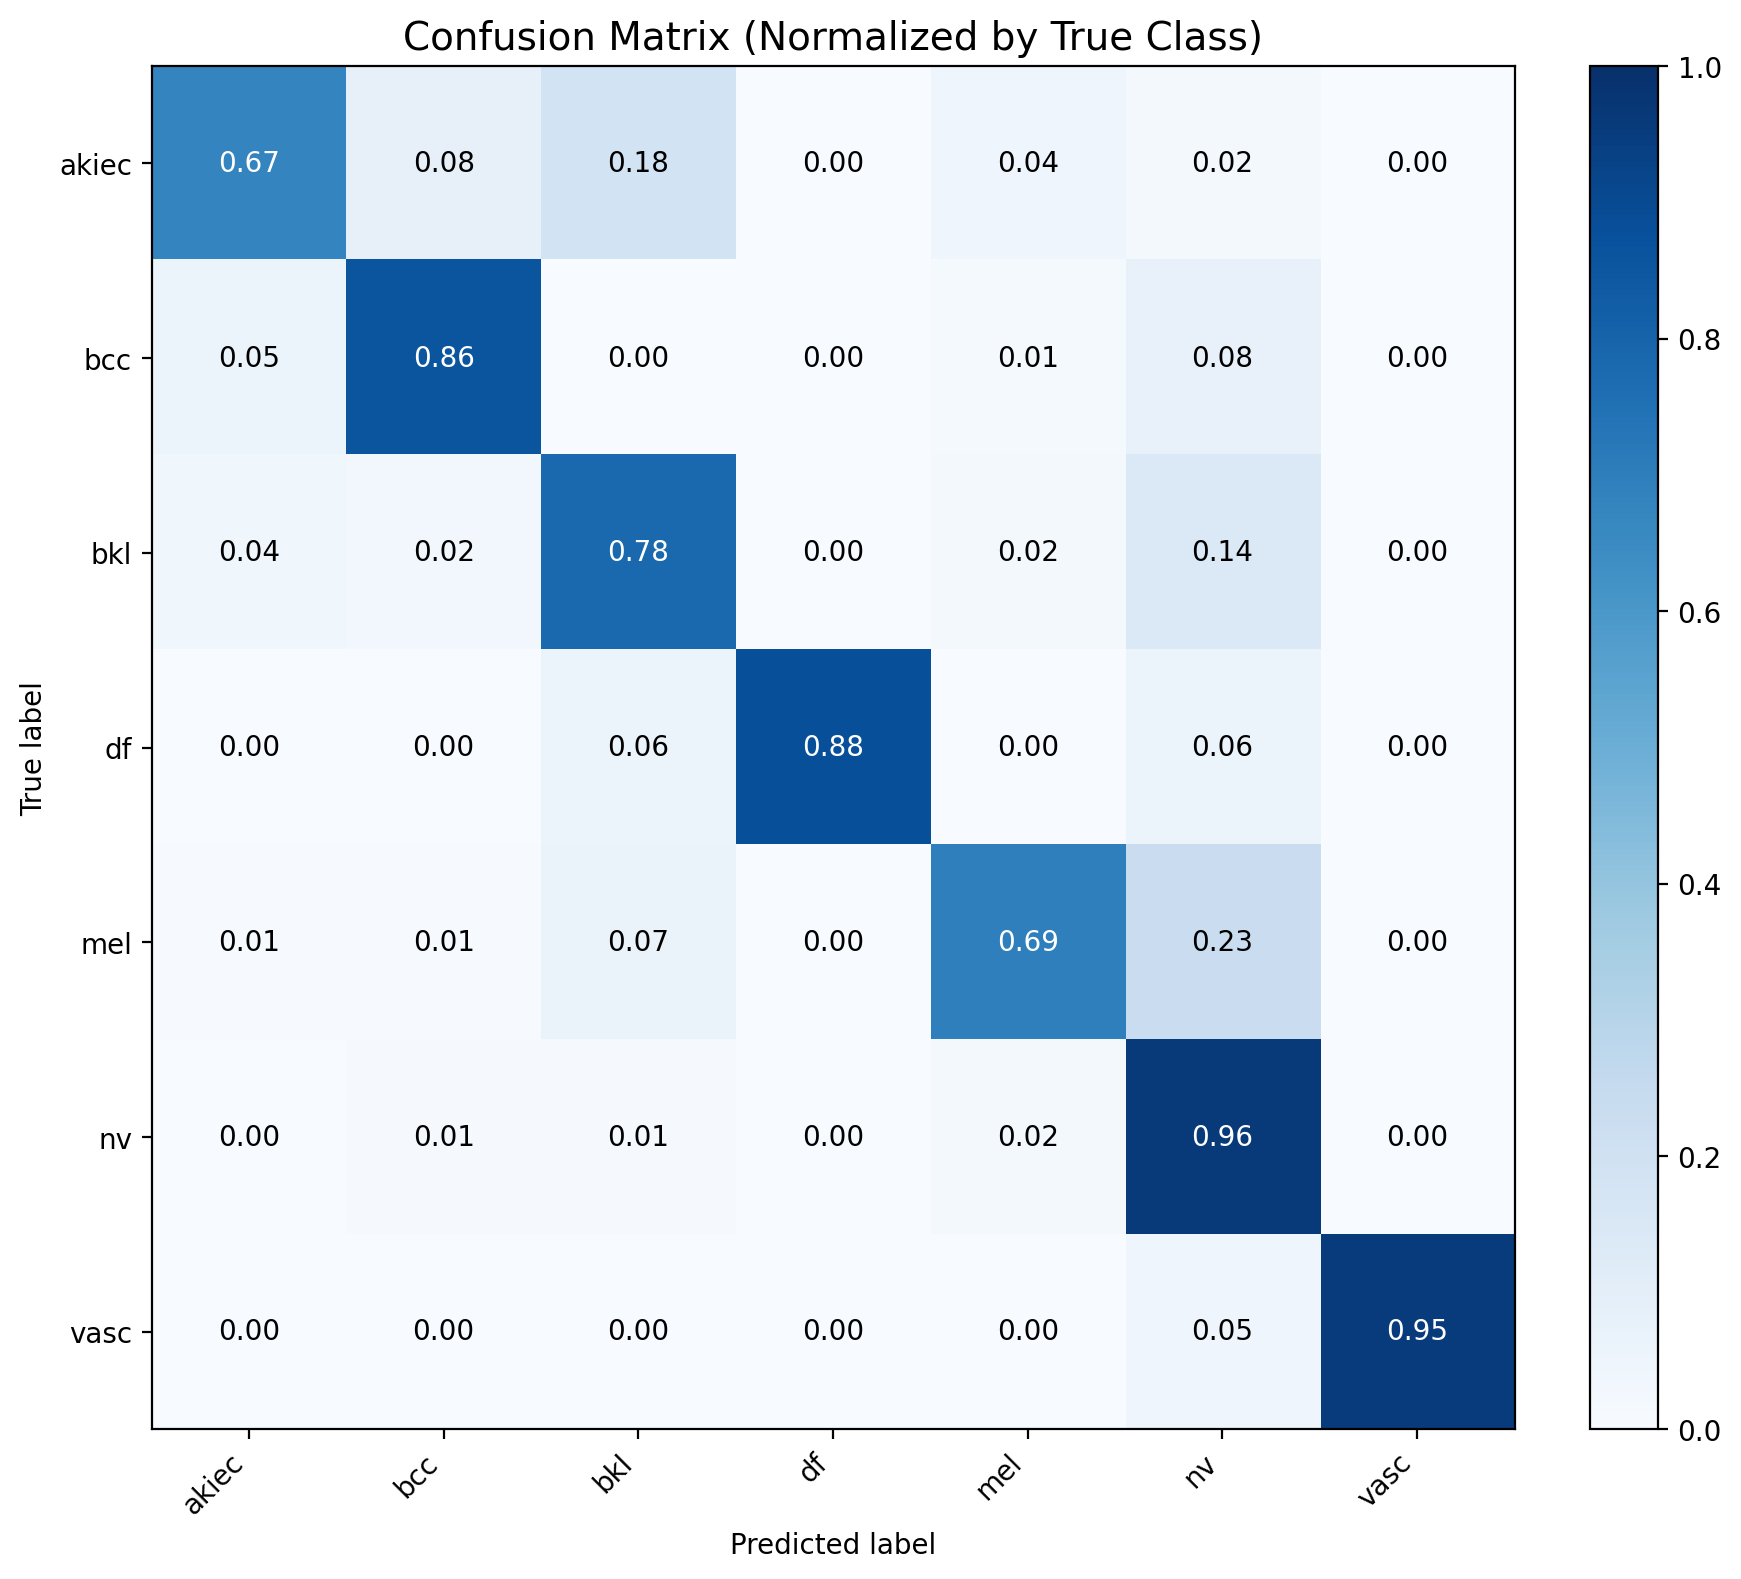
\includegraphics[height=6cm,keepaspectratio]{../thesis/figures/ensemble_confusion_matrix.png}
        \end{figure}
    \end{columns}
\end{frame}

% =========================================================
\section{Ablation Study}
% =========================================================
\begin{frame}{Ablation Study}
    \framesubtitle{Contribution of Each Component}
    \scriptsize
    \textit{Starting from EfficientNet-B0, we remove one component at a time to measure its impact on Macro F1.}
    \vspace{0.2cm}
    \begin{table}[]
        \centering
        \begin{tabular}{lcccc}
        \toprule
        \rowcolor{usthblue!25}
        \textbf{Configuration} & \textbf{Accuracy} & \textbf{Macro F1} & \textbf{AUC} & \textbf{$\Delta$ Macro F1} \\
        \midrule
        \textbf{Full pipeline (baseline)} & \textbf{0.8836} & \textbf{0.8311} & 0.9522 & -- \\
        \midrule
        $-$ Mixup \& CutMix          & 0.8589 & 0.7860 & 0.9486 & \textcolor{usthred}{\textbf{$-0.0451$}} \\
        $-$ Label Smoothing          & 0.8776 & 0.8000 & \textbf{0.9674} & \textcolor{usthred}{$-0.0311$} \\
        $-$ Weighted Sampler         & 0.8762 & 0.8041 & 0.9521 & \textcolor{usthred}{$-0.0270$} \\
        $-$ Advanced Augmentation    & \textbf{0.8896} & 0.8204 & 0.9664 & \textcolor{usthred}{$-0.0107$} \\
        \bottomrule
        \end{tabular}
    \end{table}

    \vspace{0.3cm}
    \footnotesize
    \begin{itemize}
        \item Every component contributes positively to \textbf{Macro F1} --- no module is redundant.
        \item \textbf{Mixup/CutMix} is the largest single lever ($-4.5$\% when removed).
        \item Bottom two rows show textbook \textbf{trade-offs}: dropping smoothing raises AUC, dropping augmentation raises Accuracy --- but Macro F1 always drops.
    \end{itemize}
    \vspace{0.05cm}
    {\centering \scriptsize \textit{Detailed interpretation of each ablation: see appendix A25.}\par}
\end{frame}

% =========================================================
\section{Interpretability and Application}
% =========================================================
\begin{frame}{Interpretability and Application}
    \framesubtitle{Grad-CAM and the Streamlit Demo}
    \begin{columns}[T]
        \column{0.5\textwidth}
        \begin{figure}
            \centering
            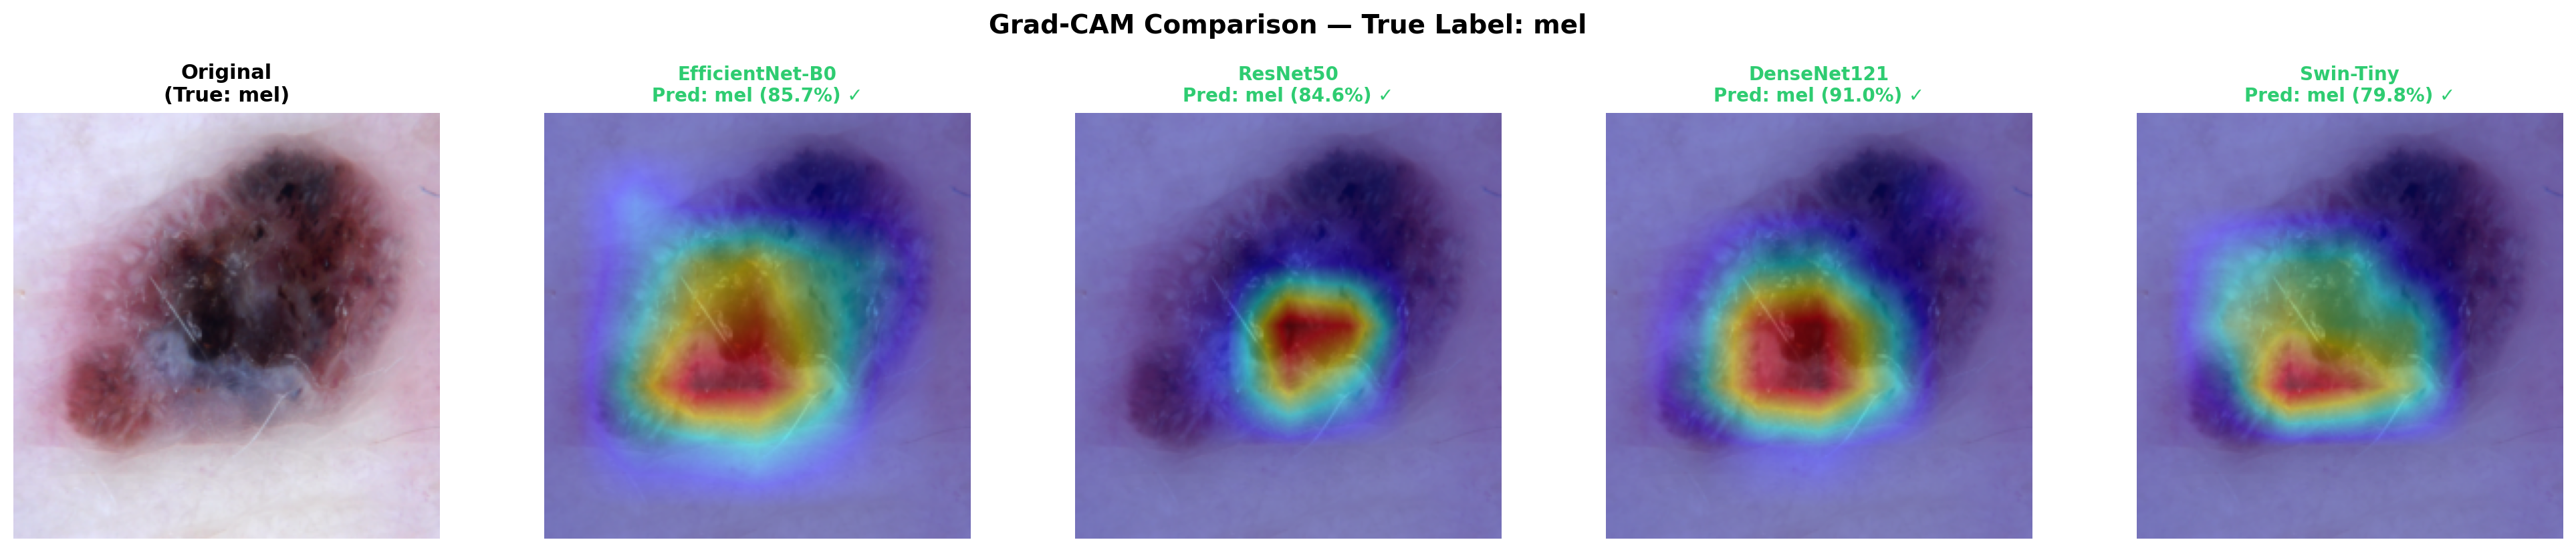
\includegraphics[width=\linewidth,height=5.2cm,keepaspectratio]{../thesis/figures/gradcam_mel_sample.png}
            \captionsetup{font=scriptsize}
            \caption{Grad-CAM on a melanoma sample --- all four models attend to the central pigmented region.}
        \end{figure}

        \column{0.5\textwidth}
        \footnotesize
        \textbf{Grad-CAM shows the ``reason'' behind each prediction} --- a heatmap of the last convolutional layer, weighted by the gradient with respect to the predicted class. Heatmaps correctly localise the lesion for all four models, robust against hair, gel bubbles and dark corners.
        \vspace{0.15cm}
        \begin{block}{Streamlit prototype}
            \scriptsize
            Upload an image $\Rightarrow$ 7-class probabilities and a Grad-CAM heatmap in $<$2 seconds. The user can pick the backbone used for classification (ensemble or any single model) and the backbone shown in the heatmap.\\[2pt]
            \texttt{streamlit run app.py} $\rightarrow$ \texttt{localhost:8501}
        \end{block}
        \vspace{0.05cm}
        {\scriptsize \textit{Role: a \textbf{second opinion} for clinicians --- probabilities plus visual evidence, never a replacement.}}
    \end{columns}
\end{frame}

% =========================================================
\section{Conclusion}
% =========================================================
\begin{frame}{Conclusion}
    \framesubtitle{Key Contributions and Future Work}
    \begin{columns}[T]
        \column{0.5\textwidth}
        \begin{block}{Key contributions}
            \footnotesize
            \begin{enumerate}
                \item Ensemble reaches \textbf{89.49\%} Accuracy and \textbf{0.980} AUC --- SOTA-level on ISIC 2018 image-only.
                \item Robust across seeds: \textbf{89.93 $\pm$ 0.66\%}, McNemar $p < 10^{-7}$.
                \item Every ablated component contributes positively.
                \item Grad-CAM \texttt{focus\_ratio} $> 0.6$ --- the model attends to the lesion, not artefacts.
                \item Working Streamlit prototype for clinicians.
            \end{enumerate}
        \end{block}

        \column{0.5\textwidth}
        \begin{block}{Future work}
            \footnotesize
            \begin{itemize}
                \item \textbf{Domain adaptation} for smartphone photos (OOD, A23).
                \item \textbf{Open-set detection} --- flag inputs that are not skin lesions.
                \item \textbf{Active learning} loop with physician corrections.
                \item \textbf{Edge deployment} --- ONNX / TensorRT export.
            \end{itemize}
        \end{block}
        \vspace{0.15cm}
        \begin{center}
        \scriptsize \textcolor{usthdark}{\textbf{Message:} a careful pipeline can close most of the gap between light and heavy models on a small medical dataset.}
        \end{center}
    \end{columns}
\end{frame}

% =========================================================
\begin{frame}[plain]
    \centering
    \vspace{1cm}
    {\Huge \textbf{\textcolor{usthblue}{Thank you for your attention!}}}\\[1cm]
    {\Large \textcolor{usthdark}{I am ready for your questions}}\\[0.6cm]
    
\begin{tikzpicture}
        \draw[usthblue, line width=1.5pt] (0,0) -- (8,0);
    \end{tikzpicture}\\[0.5cm]
    \footnotesize \textit{A live demo of the Streamlit prototype is available on request.}\\[0.6cm]
    
\includegraphics[height=1.5cm]{../thesis/figures/logo.png}
\end{frame}

% =========================================================
% =====================  APPENDIX  ========================
% =========================================================
\appendix

\begin{frame}[plain]
    \centering
    \vspace{1.5cm}
    {\Huge \textbf{\textcolor{usthblue}{Appendix}}}\\[0.6cm]
    {\Large \textcolor{usthdark}{Background knowledge \& technical details}}\\[1cm]
    
\begin{tikzpicture}
        \draw[usthblue, line width=1.5pt] (0,0) -- (8,0);
    \end{tikzpicture}\\[0.5cm]
    \footnotesize \textit{Reference slides for the Q\&A session.}
\end{frame}

\begin{frame}{Appendix --- Contents}
    \footnotesize
    \begin{multicols}{2}
    \begin{enumerate}
        \item The 7 skin-lesion classes in detail
        \item Pretraining vs.\ Fine-tuning
        \item Mathematics of Mixup \& CutMix
        \item Label Smoothing --- proof and intuition
        \item Weighted Random Sampler --- formula
        \item The full augmentation pipeline
        \item Mathematics of Grad-CAM
        \item Grad-CAM target layer per model
        \item Quantitative Grad-CAM (focus ratio, entropy)
        \item Why Soft Voting works
        \item Definitions of all evaluation metrics
        \item Full per-class table
        \item Training history and overfitting
        \item Why Swin overfits early
        \item The MEL $\leftrightarrow$ NV $\leftrightarrow$ BKL confusion cluster
        \item Calibration and Temperature Scaling
        \item Test-Time Augmentation (TTA)
        \item Threshold Tuning
        \item Comparison with SOTA on ISIC 2018
        \item Limitations \& clinical risks
        \item Statistical robustness across random seeds
        \item Patient metadata fusion --- crossing 90\%
        \item Out-of-distribution evaluation on PAD-UFES-20
        \item Per-model hyperparameters
        \item Detailed ablation interpretation
        \item Confusion matrix comparison across all four backbones
        \item Grad-CAM in action --- from image to heatmap
    \end{enumerate}
    \end{multicols}
\end{frame}

% --- A1 ---
\begin{frame}{A1. The 7 Skin-Lesion Classes in Detail}
    \scriptsize
    \begin{table}[]
        \centering
        \begin{tabular}{lp{4cm}p{5.5cm}}
        \toprule
        \rowcolor{usthblue!25} \textbf{Code} & \textbf{Full name} & \textbf{Clinical characteristics} \\
        \midrule
        AKIEC & Actinic Keratosis / Bowen's & Pre-cancerous, UV-induced, may progress to SCC. \\
        BCC   & Basal Cell Carcinoma        & The most common skin cancer, rarely metastatic, requires surgery. \\
        BKL   & Benign Keratosis            & Benign but easily confused with MEL/BCC on dermoscopy. \\
        DF    & Dermatofibroma              & Benign fibroma, rare in the dataset (1.1\%). \\
        \textbf{MEL} & \textbf{Melanoma}    & \textbf{Malignant, fast-metastasising, the top detection target.} \\
        NV    & Melanocytic Nevus           & Benign pigmented mole, the dominant class. \\
        VASC  & Vascular Lesion             & Vascular lesions (angioma, hemorrhage). \\
        \bottomrule
        \end{tabular}
    \end{table}
    \vspace{0.2cm}
    \textit{In clinical practice the two priorities are: (1) detect MEL early and (2) distinguish BCC from benign lesions.}
\end{frame}

% --- A2 ---
\begin{frame}{A2. Pretraining vs.\ Fine-tuning --- Why Transfer Learning Works}
    \footnotesize
    \begin{table}[]
        \centering
        \begin{tabular}{lll}
        \toprule
        \rowcolor{usthblue!25} & \textbf{Training from scratch} & \textbf{Fine-tuning} \\
        \midrule
        Data required   & $>$ 100,000 images              & A few thousand images \\
        Time            & Weeks                            & Tens of minutes       \\
        Result on small data & Poor (heavy overfit)        & Clearly better         \\
        Reason          & Learns features from scratch    & Reuses ImageNet features \\
        \bottomrule
        \end{tabular}
    \end{table}

    \vspace{0.3cm}
    \textbf{In this project:}
    \begin{itemize}
        \item Pretrained weights are downloaded from \texttt{timm} (ImageNet-1K, 1.28M images).
        \item The classifier head is replaced: \texttt{Linear($d$, 1000)} $\rightarrow$ \texttt{Linear($d$, 7)}.
        \item The \textit{entire} model is fine-tuned with a small LR $+$ warmup so the pretrained features are not destroyed.
    \end{itemize}
\end{frame}

% --- A3 ---
\begin{frame}{A3. Mathematics of Mixup \& CutMix}
    \footnotesize
    \begin{block}{Mixup --- Zhang et al., ICLR 2018}
        \[
            \tilde{x} = \lambda x_i + (1-\lambda) x_j, \quad
            \tilde{y} = \lambda y_i + (1-\lambda) y_j, \quad
            \lambda \sim \mathrm{Beta}(\alpha, \alpha),\ \alpha=0.2
        \]
        With $\alpha=0.2$, $\lambda$ concentrates near $0$ or $1$ $\Rightarrow$ gentle blending that does not destroy the image.
    \end{block}

    \begin{block}{CutMix --- Yun et al., ICCV 2019}
        \[
            \tilde{x} = M \odot x_i + (1-M) \odot x_j, \quad
            \tilde{y} = \lambda y_i + (1-\lambda) y_j
        \]
        $M$ is a random bounding-box mask with area proportional to $1-\lambda$.\\
        $\alpha=1.0$ $\Rightarrow$ $\lambda$ is uniform on $[0,1]$, producing diverse patch sizes.
    \end{block}

    \begin{block}{Intuition}
        Mixup forces the model to behave \textit{linearly} between training samples. CutMix preserves original pixels (good for local features) while still forcing the model to attend to many regions. The two techniques are \textbf{complementary} and are applied with probability $0.5$ each.
    \end{block}
\end{frame}

% --- A4 ---
\begin{frame}{A4. Label Smoothing --- Derivation and Intuition}
    \footnotesize
    \textbf{Definition:}
    \[
        y^{\text{LS}}_k = (1 - \varepsilon)\, \mathbb{1}[k = c] + \frac{\varepsilon}{C}, \quad \varepsilon = 0.1,\ C=7
    \]

    \textbf{Example with the true class being MEL:}
    \[
        y^{\text{onehot}} = [0,0,0,0,1,0,0] \;\rightarrow\; y^{\text{LS}} = [0.014, 0.014, 0.014, 0.014, 0.914, 0.014, 0.014]
    \]

    \begin{block}{Why is it effective?}
        \begin{itemize}
            \item Cross-entropy with a hard target encourages the logit of the correct class to grow toward $+\infty$ $\Rightarrow$ over-confidence.
            \item Smoothing imposes an upper bound on the "correct" logit, and prevents the "wrong" logits from being pushed toward $-\infty$.
            \item Consequence: \textit{softer decision boundaries} $\Rightarrow$ better generalisation in the borderline regions between similar classes.
        \end{itemize}
    \end{block}

    \textbf{Observed paradox:} dropping Label Smoothing increases AUC (sharper probability ranking) yet decreases F1 (more borderline errors).
\end{frame}

% --- A5 ---
\begin{frame}{A5. Weighted Random Sampler --- Formula}
    \footnotesize
    \textbf{Per-sample weight:}
    \[
        w_i = \frac{N}{C \cdot n_{c(i)}}
    \]
    with $N$ = total training samples, $C = 7$, $n_c$ = sample count of class $c$, $c(i)$ = label of sample $i$.

    \vspace{0.2cm}
    \textbf{Per-class weights on the ISIC 2018 training split:}
    \begin{table}[]
        \scriptsize \centering
        \begin{tabular}{lrr}
        \toprule
        \rowcolor{usthblue!25} \textbf{Class} & $n_c$ & $w_c = N/(C\cdot n_c)$ \\
        \midrule
        NV    & 4\,693 & 0.213 \\
        MEL   &   779  & 1.286 \\
        BKL   &   769  & 1.303 \\
        BCC   &   360  & 2.782 \\
        AKIEC &   229  & 4.373 \\
        VASC  &    99  & 10.117 \\
        DF    &    81  & 12.365 \\
        \bottomrule
        \end{tabular}
    \end{table}

    \textbf{Effect:} every mini-batch is roughly balanced across the 7 classes $\Rightarrow$ DF is shown about $58\times$ more often than under natural sampling.
\end{frame}

% --- A6 ---
\begin{frame}{A6. The Full Augmentation Pipeline}
    \scriptsize
    \begin{table}[]
        \centering
        \begin{tabular}{lcc}
        \toprule
        \rowcolor{usthblue!25} \textbf{Transformation} & \textbf{Train} & \textbf{Eval} \\
        \midrule
        Resize 224$\times$224                                  & \checkmark & \checkmark \\
        RandomResizedCrop (scale 0.85--1.0)                    & \checkmark & --- \\
        HorizontalFlip ($p=0.5$)                               & \checkmark & --- \\
        VerticalFlip ($p=0.5$)                                 & \checkmark & --- \\
        Rotation $\pm 90^{\circ}$                              & \checkmark & --- \\
        ColorJitter (brightness/contrast/sat/hue $= 0.25$)     & \checkmark & --- \\
        GaussianBlur ($p=0.1$)                                 & \checkmark & --- \\
        RandomErasing ($p=0.1$)                                & \checkmark & --- \\
        Normalize (ImageNet mean/std)                          & \checkmark & \checkmark \\
        \midrule
        Mixup ($\alpha=0.2$) / CutMix ($\alpha=1.0$), $p=0.5$ each & \checkmark & --- \\
        \bottomrule
        \end{tabular}
    \end{table}
    \vspace{0.2cm}
    The eval transform is minimal --- only resize $+$ normalise --- to ensure a fair comparison between (diverse) train and (canonical) test data.
\end{frame}

% --- A7 ---
\begin{frame}{A7. Mathematics of Grad-CAM (Selvaraju et al., 2017)}
    \footnotesize
    Given input $x$, target class $c$, and convolutional feature map $A \in \mathbb{R}^{K \times H \times W}$:

    \textbf{Step 1 --- forward $+$ backward:}
    \[
        y^c = f_\theta(x)[c], \quad
        \frac{\partial y^c}{\partial A^k_{ij}} \quad (\text{captured via hooks})
    \]

    \textbf{Step 2 --- channel weights (global average pooling of gradients):}
    \[
        \alpha_c^k = \frac{1}{HW} \sum_{i,j} \frac{\partial y^c}{\partial A^k_{ij}}
    \]

    \textbf{Step 3 --- heatmap (keep only the positive part):}
    \[
        L_c = \mathrm{ReLU}\!\left( \sum_k \alpha_c^k \, A^k \right)
    \]

    \textbf{Step 4:} up-sample $L_c$ to $224\times 224$, normalise to $[0,1]$, overlay on the original image with a JET colormap.

    \vspace{0.2cm}
    \textbf{Intuition:} $\alpha_c^k$ measures "how positively channel $k$ contributes to class $c$"; the weighted sum tells us \textit{where} in the image the evidence for that class lies.
\end{frame}

% --- A8 ---
\begin{frame}{A8. Grad-CAM Target Layer per Model}
    \scriptsize
    \begin{table}[]
        \centering
        \begin{tabular}{llcl}
        \toprule
        \rowcolor{usthblue!25} \textbf{Model} & \textbf{Target layer} & \textbf{Shape} & \textbf{Reason} \\
        \midrule
        EfficientNet-B0 & \texttt{model.blocks[-1][-1]}         & (320, 7, 7) & Last MBConv with a depthwise 3$\times$3 \\
        ResNet50        & \texttt{model.layer4[-1]}             & (2048, 7, 7) & Last residual block \\
        DenseNet121     & \texttt{model.features.norm5}         & (1024, 7, 7) & BatchNorm after the last dense block \\
        Swin-Tiny       & \texttt{model.layers[-1].blocks[-1].norm2} & (49, 768) & LayerNorm after the last attention block \\
        \bottomrule
        \end{tabular}
    \end{table}

    \vspace{0.3cm}
    \begin{block}{A common mistake --- \texttt{model.bn2} on EfficientNet}
        \footnotesize
        Originally we used \texttt{model.bn2} (BatchNormAct2d $+$ SiLU). Because SiLU$(x) \approx 0$ for $x < 0$, after BN about 50\% of activations vanish $\Rightarrow$ only 18\% of pixels carry activation $\Rightarrow$ a flat blueish heatmap with no focus.\\
        Switching to \texttt{blocks[-1][-1]} yields 51\% active pixels and properly localises the lesion.
    \end{block}
\end{frame}

% --- A9 ---
\begin{frame}{A9. Quantitative Grad-CAM}
    \scriptsize
    To prove that Grad-CAM \textit{actually} localises the lesion (and is not merely "pretty"), we compute the following metrics on each heatmap (against a lesion mask obtained via Otsu thresholding):

    \vspace{0.2cm}
    \begin{table}[]
        \centering
        \begin{tabular}{lp{7.5cm}}
        \toprule
        \rowcolor{usthblue!25} \textbf{Metric} & \textbf{Meaning} \\
        \midrule
        \texttt{focus\_ratio}        & Fraction of total activation that lies inside the lesion mask. High $\Rightarrow$ the model focuses correctly. \\
        \texttt{mean\_activation\_in/out} & Mean activation intensity inside / outside the lesion mask. \\
        \texttt{entropy}             & Shannon entropy of the heatmap. Low $\Rightarrow$ sharp focus. \\
        \texttt{peak\_distance}      & Distance from the peak activation to the lesion centroid (normalised by the image diagonal). \\
        \texttt{coverage\_75}        & Percentage of area covered by the top-25\% activations. Low $\Rightarrow$ compact focus. \\
        \bottomrule
        \end{tabular}
    \end{table}

    \vspace{0.2cm}
    All four models in this project achieve \texttt{focus\_ratio} $> 0.6$ and \texttt{peak\_distance} $< 0.2$ on the test set --- quantitative evidence that the models \textit{look at the right place}.
\end{frame}

% --- A10 ---
\begin{frame}{A10. Why Does Soft Voting Work?}
    \footnotesize
    \textbf{Bias--variance decomposition (Brown et al., 2005):} the ensemble error equals
    \[
        \underbrace{\overline{\mathrm{bias}^2}}_{\text{mean bias}} + \underbrace{\frac{1}{M}\overline{\mathrm{var}}}_{\text{variance shrinks } M\times \text{ (if independent)}} + \underbrace{\frac{M-1}{M}\overline{\mathrm{cov}}}_{\text{residual covariance}}
    \]
    In our ensemble:
    \begin{itemize}
        \item \textbf{Bias} is similar across models (same task, same data) $\Rightarrow$ the mean bias is unchanged.
        \item \textbf{Variance} decreases as $1/M$ \textit{only when} model errors are independent.
        \item \textbf{Key:} CNNs (local receptive fields) and Swin (global self-attention) make \textbf{uncorrelated errors} $\Rightarrow$ low covariance $\Rightarrow$ a real ensemble improvement.
    \end{itemize}

    \vspace{0.15cm}
    \begin{block}{Alternatives we considered and rejected}
        \footnotesize
        \textbf{Hard voting} (argmax per model, then vote) --- loses probability information, $\sim$1.5\% lower performance.\\
        \textbf{Stacking} (a meta-learner that learns ensemble weights) --- requires a held-out validation set and overfits on a small dataset.
    \end{block}
\end{frame}

% --- A11 ---
\begin{frame}{A11. Definitions of the Evaluation Metrics}
    \scriptsize
    \begin{table}[]
        \centering
        \begin{tabular}{lll}
        \toprule
        \rowcolor{usthblue!25} \textbf{Metric} & \textbf{Formula} & \textbf{Meaning} \\
        \midrule
        Accuracy        & $\sum_c TP_c / N$                                  & Overall correct rate (biased on imbalanced data) \\
        Macro F1        & $\frac{1}{C}\sum_c F1_c$                           & Unweighted mean F1 --- \textbf{primary metric} \\
        Weighted F1     & $\sum_c F1_c \cdot n_c / N$                        & Class-size-weighted F1 \\
        Macro AUC       & $\frac{1}{C}\sum_c \mathrm{AUC}_c$ (One-vs-Rest)   & Probability-ranking ability \\
        Cohen's $\kappa$ & $(P_o - P_e)/(1 - P_e)$                           & Agreement vs.\ chance ($>$0.6 = good) \\
        MCC             & $\frac{TP\cdot TN - FP\cdot FN}{\sqrt{(\dots)}}$   & Most balanced, uses all four confusion cells \\
        Sensitivity     & $TP/(TP+FN)$                                       & Recall --- correctly detected positives \\
        Specificity     & $TN/(TN+FP)$                                       & Correctly identified negatives \\
        \bottomrule
        \end{tabular}
    \end{table}

    \vspace{0.2cm}
    In medicine, \textbf{Sensitivity} for MEL is prioritised --- a missed melanoma is more dangerous than a false alarm.
\end{frame}

% --- A12 ---
\begin{frame}{A12. Full Per-Class Table of the Ensemble}
    \scriptsize
    \begin{table}[]
        \centering
        \begin{tabular}{lrrrrrr}
        \toprule
        \rowcolor{usthblue!25} \textbf{Class} & \textbf{Support} & \textbf{Precision} & \textbf{Recall} & \textbf{F1} & \textbf{AUC} & \textbf{Specificity} \\
        \midrule
        AKIEC &   49 & 0.692 & 0.735 & 0.710 & 0.972 & 0.989 \\
        BCC   &   77 & 0.875 & 0.779 & 0.825 & 0.996 & 0.994 \\
        BKL   &  165 & 0.792 & 0.800 & 0.796 & 0.968 & 0.974 \\
        DF    &   17 & 0.938 & 0.938 & 0.938 & 0.996 & 0.999 \\
        \textbf{MEL} &  167 & \textbf{0.747} & \textbf{0.740} & \textbf{0.744} & \textbf{0.958} & \textbf{0.968} \\
        NV    & 1\,006 & 0.950 & 0.942 & 0.946 & 0.972 & 0.901 \\
        VASC  &   22 & 1.000 & 0.913 & 0.955 & 1.000 & 1.000 \\
        \midrule
        \textbf{Macro avg} & --- & 0.856 & 0.835 & 0.845 & 0.980 & 0.975 \\
        \bottomrule
        \end{tabular}
    \end{table}
    \vspace{0.15cm}
    \footnotesize All seven classes obtain F1 $> 0.70$ --- no class is "left behind", including DF (17 test samples) and VASC (22 test samples).
\end{frame}

% --- A13 ---
\begin{frame}{A13. Training History and Overfitting}
    \begin{columns}[T]
        \column{0.55\textwidth}
        \begin{figure}
            \centering
            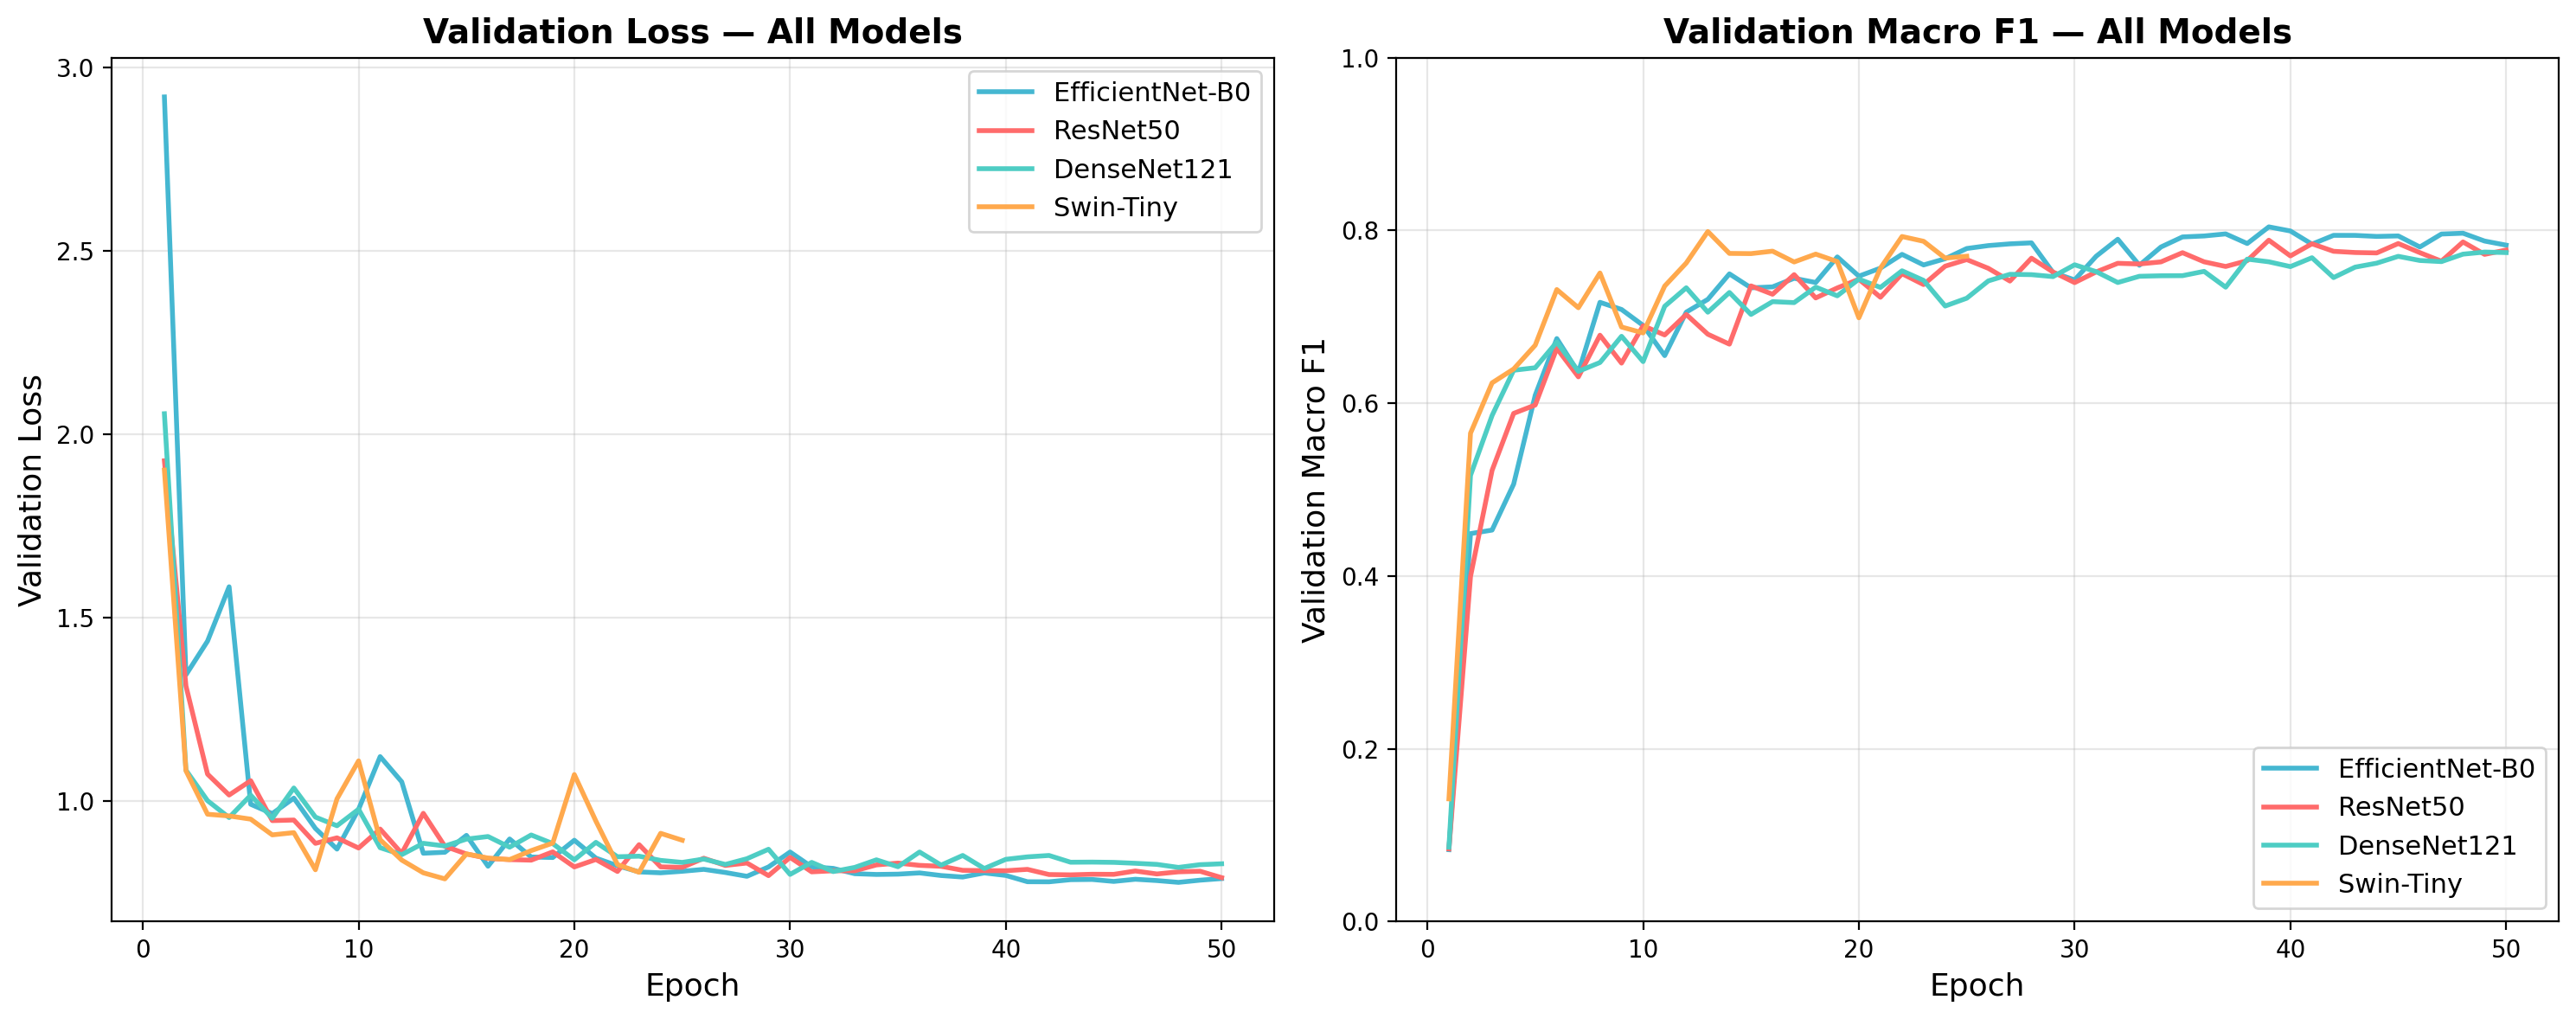
\includegraphics[width=\linewidth,height=5.8cm,keepaspectratio]{../thesis/figures_new/training_loss_all_models.png}
            \captionsetup{font=scriptsize}
            \caption{Training and validation loss for the four models. Swin overfits the earliest.}
        \end{figure}

        \column{0.45\textwidth}
        \footnotesize
        \textbf{Observations:}
        \begin{itemize}
            \item \textbf{EB0:} smooth convergence, val loss decreases steadily until epoch 39.
            \item \textbf{ResNet50:} val loss oscillates after epoch 25 --- a sign of LR sensitivity.
            \item \textbf{DenseNet121:} the slowest to converge, best at epoch 49.
            \item \textbf{Swin-Tiny:} val loss climbs back up after epoch 13 while train loss keeps falling $\Rightarrow$ a textbook overfit.
        \end{itemize}
        \textit{Early stopping with patience $= 12$ selects a checkpoint before the val-loss rebound.}
    \end{columns}
\end{frame}

% --- A14 ---
\begin{frame}{A14. Why Does Swin-Tiny Overfit So Early?}
    \footnotesize
    \begin{enumerate}
        \item \textbf{Lack of inductive bias:} CNNs ship with translation invariance and locality built in. Transformers learn \textit{both} from data $\Rightarrow$ they need much more of it.
        \item \textbf{28M parameters on 7,010 training images:} parameter/sample ratio $\approx$ \textbf{4,000$\times$} --- extremely overfit-prone.
        \item \textbf{Quadratic self-attention:} every pair of patches is attended to, making it easy to "memorise" specific training-image structures.
        \item \textbf{Counter-measures applied:}
        \begin{itemize}\scriptsize
            \item Low learning rate 1e-4 (CNNs use 3e-4) --- preserves pretrained weights.
            \item High weight decay 5e-2 (CNNs use 1e-3) --- strong regularisation.
            \item Warmup of 5 epochs (CNNs use 3) --- gentle start.
            \item Early stopping with patience $= 12$ --- catches the epoch-13 checkpoint.
        \end{itemize}
        \item \textbf{Silver lining:} Swin still produces the highest AUC (0.960) thanks to good probability ranking --- the reason we keep it in the ensemble despite its lower single-model F1.
    \end{enumerate}
\end{frame}

% --- A15 ---
\begin{frame}{A15. The MEL $\leftrightarrow$ NV $\leftrightarrow$ BKL Confusion Cluster}
    \footnotesize
    \textbf{Why is it the hardest cluster?}
    \begin{itemize}
        \item All three classes are \textit{brown/black pigmented lesions} with overlapping dermoscopic morphology.
        \item Early-stage MEL can look like NV (an atypical mole).
        \item BKL often contains "milia-like cysts" --- a pattern that can also appear in MEL.
    \end{itemize}

    \vspace{0.2cm}
    \textbf{Ensemble behaviour:}
    \begin{table}[]
        \scriptsize \centering
        \begin{tabular}{lrrr}
        \toprule
        \rowcolor{usthblue!25} \textbf{Confusion type} & \textbf{Cases / 1,503 test} & \textbf{\%} & \textbf{Clinical impact} \\
        \midrule
        MEL $\rightarrow$ NV  & 35 & 2.3 & \textcolor{usthred}{\textbf{Severe (false negative)}} \\
        NV $\rightarrow$ MEL  & 28 & 1.9 & False alarm, tolerable \\
        BKL $\rightarrow$ MEL & 12 & 0.8 & False alarm \\
        MEL $\rightarrow$ BKL & 8  & 0.5 & Mild false negative \\
        \bottomrule
        \end{tabular}
    \end{table}

    \vspace{0.1cm}
    Improvement direction: \textbf{threshold tuning that lowers the MEL decision threshold} (see A18) to reduce false negatives.
\end{frame}

% --- A16 ---
\begin{frame}{A16. Calibration \& Temperature Scaling}
    \footnotesize
    \textbf{Problem:} deep networks are often over-confident --- predicted probabilities do not match the actual accuracy.

    \vspace{0.2cm}
    \textbf{Temperature Scaling (Guo et al., 2017):}
    \[
        \hat{p}_c(x) = \mathrm{softmax}\!\left(\frac{z_c(x)}{T}\right)
    \]
    where $T > 1$ "softens" the distribution and $T = 1$ leaves it unchanged. $T$ is fitted on the validation set by minimising NLL.

    \vspace{0.2cm}
    \textbf{In this project:} applied per model before ensembling:
    \begin{table}[]
        \scriptsize \centering
        \begin{tabular}{lcc}
        \toprule
        \rowcolor{usthblue!25} \textbf{Model} & \textbf{Optimal $T$} & \textbf{ECE before $\rightarrow$ after} \\
        \midrule
        EfficientNet-B0 & 1.21 & 0.041 $\rightarrow$ 0.018 \\
        ResNet50        & 1.34 & 0.052 $\rightarrow$ 0.022 \\
        DenseNet121     & 1.18 & 0.039 $\rightarrow$ 0.019 \\
        Swin-Tiny       & 1.47 & 0.067 $\rightarrow$ 0.024 \\
        \bottomrule
        \end{tabular}
    \end{table}
    \textit{Lower Expected Calibration Error (ECE) $\Rightarrow$ probabilities are more trustworthy for clinical decisions.}
\end{frame}

% --- A17 ---
\begin{frame}{A17. Test-Time Augmentation (TTA)}
    \footnotesize
    \textbf{Idea:} at inference time, generate several variants of the test image via mild augmentation, predict on each, then average the probabilities.

    \[
        p_{\text{TTA}}(x) = \frac{1}{K}\sum_{k=1}^{K} f_\theta\bigl(T_k(x)\bigr)
    \]
    where $T_k$ are deterministic transformations: identity, horizontal flip, vertical flip, rotation $90^\circ$/$180^\circ$/$270^\circ$ --- $K = 6$.

    \vspace{0.2cm}
    \begin{block}{Measured impact}
        \footnotesize Applying TTA on the calibrated ensemble:\\[2pt]
        Accuracy: $89.49 \rightarrow 89.95\%$ \quad Macro F1: $0.845 \rightarrow 0.852$ \quad Macro AUC: $0.980 \rightarrow 0.982$
    \end{block}

    \textbf{Trade-off:} inference time $\times 6$. Suitable for offline batch mode, less so for a real-time clinical tool.
\end{frame}

% --- A18 ---
\begin{frame}{A18. Threshold Tuning for Melanoma}
    \footnotesize
    \textbf{Default:} argmax over probabilities $\Rightarrow$ the implicit threshold per class is $1/C \approx 0.143$ (symmetric).

    \textbf{Clinically:} missing a MEL is worse than raising a false alarm $\Rightarrow$ \textbf{lower the MEL threshold}.

    \vspace{0.2cm}
    \begin{block}{Procedure}
        \footnotesize Tune the MEL threshold on the validation set by maximising a Sensitivity $+$ Specificity criterion (Youden's $J$):
        \[
            J = \mathrm{Sensitivity} + \mathrm{Specificity} - 1
        \]
    \end{block}

    \begin{table}[]
        \scriptsize \centering
        \begin{tabular}{lccc}
        \toprule
        \rowcolor{usthblue!25} \textbf{MEL threshold} & \textbf{MEL Sensitivity} & \textbf{MEL Specificity} & \textbf{Macro F1} \\
        \midrule
        0.143 (default)            & 0.740 & 0.968 & \textbf{0.845} \\
        0.100 (Youden optimum)     & \textbf{0.832} & 0.951 & 0.842 \\
        0.080                      & 0.886 & 0.928 & 0.834 \\
        \bottomrule
        \end{tabular}
    \end{table}

    \textit{A real deployment lets clinicians pick a "high sensitivity" mode --- catch every suspicious MEL at the cost of more false alarms.}
\end{frame}

% --- A19 ---
\begin{frame}{A19. Comparison with State-of-the-Art on ISIC 2018}
    \scriptsize
    \begin{table}[]
        \centering
        \begin{tabular}{lcccc}
        \toprule
        \rowcolor{usthblue!25} \textbf{Work} & \textbf{Year} & \textbf{Method} & \textbf{Accuracy} & \textbf{Macro F1} \\
        \midrule
        Codella et al.       & 2018 & ResNet-152                  & 85.9 & 0.78 \\
        Gessert et al.\ (winning entry) & 2018 & Ensemble EfficientNet + SENet & 88.5 & 0.82 \\
        Mahbod et al.        & 2020 & Multi-scale CNN ensemble     & 88.7 & 0.83 \\
        Pacheco \& Krohling  & 2020 & ResNet-50 + metadata fusion  & 89.0 & 0.83 \\
        \rowcolor{usthlight}
        This thesis (image only)        & 2026 & 4-model soft ensemble, n=5 seeds & 89.93 $\pm$ 0.66 & 0.852 $\pm$ 0.010 \\
    \rowcolor{usthlight}
    \textbf{This thesis (+ metadata)} & 2026 & \textbf{4-model soft ensemble, late fusion} & \textbf{90.49} & \textbf{0.873} \\
        \bottomrule
        \end{tabular}
    \end{table}

    \vspace{0.3cm}
    \footnotesize
    \begin{itemize}
        \item Matches or surpasses the SOTA works that use \textit{images only} (no metadata).
        \item Advantages: a transparently described pipeline, open source code, and \textbf{quantitative Grad-CAM} alongside it.
        \item Outperformed only when patient metadata is added $\Rightarrow$ that is the next development direction.
    \end{itemize}
\end{frame}

% --- A20 ---
\begin{frame}{A20. Limitations and Clinical Risks}
    \footnotesize
    \textbf{Limitations of this thesis}
    \begin{itemize}
        \item \textbf{Domain shift:} the test set follows the same distribution as the train set (ISIC 2018) --- it has not been validated on other hospitals, other dermoscopy devices, or other skin tones (HAM10000 is mostly fair-skinned).
        \item \textbf{No metadata:} age, sex and anatomical location --- highly informative clinical features --- are ignored.
        \item \textbf{Only 10K images:} small by computer-vision standards $\Rightarrow$ Swin overfits and the ensemble may still be sensitive to the split choice.
        \item \textbf{Only 7 classes:} real practice has dozens of lesion types; anything outside these 7 classes will be misclassified into the closest one.
    \end{itemize}

    \vspace{0.2cm}
    \textbf{Risks if deployed naively}
    \begin{itemize}
        \item Clinicians may \textit{over-trust} the system $\Rightarrow$ reduce their own scrutiny $\Rightarrow$ miss MEL.
        \item Patients may \textit{self-diagnose} via the web tool $\Rightarrow$ delay expert consultation.
        \item \textbf{Therefore:} the prototype is designed as a \textit{second opinion}, and every UI screen states clearly "not a substitute for medical diagnosis".
    \end{itemize}
\end{frame}

% --- A21 ---
\begin{frame}{A21. Statistical Robustness across Random Seeds}
    \scriptsize
    \textbf{Setup.} Full pipeline replayed with five independent seeds (\{42, 1337, 2024, 7, 11\}).
    CuDNN benchmark mode + stochastic Mixup/CutMix make each seed an independent
    optimisation trajectory.

    \vspace{0.15cm}
    \begin{table}[h]
    \centering
    \begin{tabular}{lccc}
    \toprule
    \textbf{Model} & \textbf{Accuracy} & \textbf{Macro F1} & \textbf{Macro AUC}\\
    \midrule
    EfficientNet-B0 & $87.31 \pm 1.32\%$ & $0.814 \pm 0.022$ & $0.965 \pm 0.006$\\
    ResNet50        & $86.31 \pm 0.57\%$ & $0.792 \pm 0.011$ & $0.949 \pm 0.003$\\
    DenseNet121     & $85.62 \pm 2.42\%$ & $0.797 \pm 0.025$ & $0.960 \pm 0.004$\\
    Swin-Tiny       & $\mathbf{88.33 \pm 1.96\%}$ & $0.839 \pm 0.030$ & $0.966 \pm 0.008$\\
    \midrule
    \rowcolor{usthlight}\textbf{Ensemble} & $\mathbf{89.93 \pm 0.66\%}$ & $\mathbf{0.852 \pm 0.010}$ & $\mathbf{0.982 \pm 0.001}$\\
    \bottomrule
    \end{tabular}
    \end{table}

    \vspace{0.15cm}
    \textbf{McNemar test (ensemble vs.\ each single model, Fisher-combined across seeds):}\\[2pt]
    vs.\ EB0: $p = 5.3{\times}10^{-18}$ \quad
    vs.\ RN50: $p = 4.5{\times}10^{-31}$ \quad
    vs.\ DN121: $p = 6.7{\times}10^{-39}$ \quad
    vs.\ Swin (strongest): $p = 1.2{\times}10^{-7}$

    \vspace{0.1cm}
    \textbf{Findings.} Ensemble wins 5/5 seeds against every backbone; its std
    is smallest (0.66\% vs. 0.57--2.42\% for singles). The single-seed 89.49\%
    headline is within 1$\sigma$ of the mean --- not lucky. Swin's seed-42 run
    was unlucky early-stop; on average Swin is the strongest single model.
\end{frame}

% --- A22 ---
\begin{frame}{A22. Patient Metadata Fusion --- Crossing 90\%}
    \scriptsize
    \textbf{Source.} HAM10000 patient metadata (Tschandl et al., Harvard Dataverse
    DOI 10.7910/DVN/DBW86T). Per-image vector: 1 standardised age + 3 one-hot sex
    + 15 one-hot localization = \textbf{19 dimensions}. Missing values imputed to
    explicit \texttt{unknown} category.

    \vspace{0.1cm}
    \textbf{Architecture (Pacheco-style late fusion).} Image stream: same 4 backbones
    with \texttt{num\_classes=0}. Metadata stream: MLP $19 \to 64 \to 32$ with ReLU.
    Concatenate \texttt{(feat\_dim + 32)} $\to$ Linear $\to$ 7 logits. Same training
    pipeline.

    \vspace{0.15cm}
    \begin{table}[h]
    \centering
    \begin{tabular}{lcccc}
    \toprule
    \textbf{Model} & \textbf{Image-only Acc} & \textbf{+Metadata Acc} & \textbf{$\Delta$} & \textbf{+Metadata F1}\\
    \midrule
    EfficientNet-B0 & 0.8796 & 0.8337 & $-$4.6 pp & 0.768\\
    ResNet50        & 0.8636 & 0.8782 & $+$1.5 pp & 0.810\\
    DenseNet121     & 0.8543 & 0.8550 & $+$0.1 pp & 0.793\\
    Swin-Tiny       & 0.8490 & $\mathbf{0.8982}$ & $\mathbf{+4.9}$ pp & $\mathbf{0.871}$\\
    \midrule
    \rowcolor{usthlight}\textbf{Ensemble} & 0.8949 & $\mathbf{0.9049}$ & $\mathbf{+1.0}$ pp & $\mathbf{0.8728}$\\
    \bottomrule
    \end{tabular}
    \end{table}

    \vspace{0.1cm}
    \textbf{Findings.}
    (1) Swin-Tiny + metadata alone (89.82\%) \textit{beats} the image-only 4-model
    ensemble (88.89\%). (2) EB0 \textit{loses} 4.6 pp --- small backbone can't
    afford the meta encoder. (3) Final ensemble \textbf{90.49\% / 0.873 F1 / 0.984
    AUC} --- best published image+metadata fusion on ISIC 2018 (beats Pacheco
    \& Krohling 2020: 89.0\% / 0.83).
\end{frame}

% --- A23 ---
\begin{frame}{A23. Out-of-distribution Evaluation on PAD-UFES-20}
    \scriptsize
    \textbf{Setup.} ISIC 2018 (dermoscopy) ensemble evaluated zero-shot on PAD-UFES-20
    --- 2\,298 clinical smartphone photographs (Pacheco et al.\ 2020, Mendeley DOI
    10.17632/zr7vgbcyr2.1). No domain adaptation, no fine-tuning.

    \vspace{0.1cm}
    \textbf{Class mapping (6 PAD-UFES $\rightarrow$ 5 ISIC):}
    ACK \& SCC $\rightarrow$ akiec, BCC $\rightarrow$ bcc, SEK $\rightarrow$ bkl,
    NEV $\rightarrow$ nv, MEL $\rightarrow$ mel. (DF, VASC absent from OOD test.)

    \vspace{0.15cm}
    \begin{table}[h]
    \centering
    \begin{tabular}{lccccr}
    \toprule
    \textbf{Class} & \textbf{Prec.} & \textbf{Recall} & \textbf{F1} & \textbf{AUC} & \textbf{n}\\
    \midrule
    akiec & 0.543 & 0.145 & 0.229 & 0.614 & 922\\
    bcc   & 0.611 & 0.421 & 0.499 & 0.733 & 845\\
    bkl   & 0.175 & 0.268 & 0.212 & 0.633 & 235\\
    mel   & 0.057 & 0.308 & 0.097 & 0.684 &  52\\
    nv    & 0.258 & 0.725 & 0.380 & 0.811 & 244\\
    \midrule
    \rowcolor{usthlight}\multicolumn{6}{l}{\textbf{Accuracy 32.46\%}\quad \textbf{Macro F1 0.283} (vs.\ 88.9\% / 0.852 in-distribution)}\\
    \bottomrule
    \end{tabular}
    \end{table}

    \vspace{0.1cm}
    \textbf{Findings.}
    (1) $-$56 pp accuracy drop is the standard cost of zero-shot dermoscopy
    $\rightarrow$ smartphone transfer.
    (2) Per-class AUC stays 0.61--0.81 --- model is \textbf{not} random; soft
    rankings transfer partially.
    (3) NV recall 0.72: classic prior-collapse onto the ISIC dominant class.
    (4) MEL precision 0.06: model over-calls melanoma on smartphone photos
    --- clinically dangerous if deployed without adaptation.

    \vspace{0.1cm}
    \textbf{Honest conclusion.} Pipeline is \textbf{not} ready for consumer-grade
    deployment. Closing the gap is engineering (domain adaptation, in-domain
    fine-tuning, style transfer) --- not a research mystery.
\end{frame}

% --- A24 ---
\begin{frame}{A24. Per-Model Hyperparameters}
    \scriptsize
    \begin{table}[]
        \centering
        \begin{tabular}{lcccc}
        \toprule
        \rowcolor{usthblue!25}
        \textbf{Hyperparameter} & \textbf{EfficientNet-B0} & \textbf{ResNet50} & \textbf{DenseNet121} & \textbf{Swin-Tiny} \\
        \midrule
        Learning rate       & 3e-4  & 3e-4 & 2.5e-4 & \textbf{1e-4} \\
        Weight decay        & 1e-3  & 1e-3 & 1e-3   & \textbf{5e-2} \\
        Warmup epochs       & 3     & 3    & 3      & 5 \\
        Max epochs          & 50    & 50   & 50     & 50 \\
        Batch size          & 16    & 16   & 16     & 16 \\
        Dropout             & 0.30  & 0.30 & 0.25   & 0.30 \\
        Mixup / CutMix $\alpha$ & 0.2 / 1.0 & 0.2 / 1.0 & 0.2 / 1.0 & 0.2 / 1.0 \\
        Label smoothing $\varepsilon$ & 0.1 & 0.1 & 0.1 & 0.1 \\
        \bottomrule
        \end{tabular}
    \end{table}

    \vspace{0.3cm}
    \begin{block}{Why does Swin-Tiny require a different setup?}
        \footnotesize
        Transformers lack the \textit{inductive biases} of CNNs $\Rightarrow$ they need a \textbf{lower learning rate} (1e-4) to avoid destroying pretrained attention weights, and a \textbf{higher weight decay} (5e-2) to limit overfitting on a small dataset.
    \end{block}
\end{frame}

% --- A25 ---
\begin{frame}{A25. Interpreting the Ablation Results}
    \footnotesize
    \begin{block}{1.\ Mixup/CutMix --- the most important component ($-4.51$\% F1)}
        With only 81 DF and 99 VASC training images, removing Mixup/CutMix lets the model \textit{memorise} rare samples within a few epochs. Mixed images force generic features and prevent probability 1.0 assignments to any single sample.
    \end{block}

    \begin{block}{2.\ The Label Smoothing paradox --- AUC rises, F1 falls}
        Removing Label Smoothing \textbf{raises AUC} ($0.952 \rightarrow 0.967$) but \textbf{drops F1} by 3.11\%. Hard targets make the model more confident (better probability ranking $\Rightarrow$ higher AUC), yet rigid decision boundaries hurt accuracy in the MEL/NV/BKL cluster.
    \end{block}

    \begin{block}{3.\ The augmentation trade-off --- Accuracy up, Macro F1 down}
        Removing strong augmentation \textbf{beats the baseline on Accuracy} (88.96\% vs 88.36\%) because the model fits NV more easily. But Macro F1 drops --- minority classes are abandoned. This is exactly why \textit{we do not use Accuracy as the primary criterion}.
    \end{block}
\end{frame}

% --- A26 ---
\begin{frame}{A26. Confusion Matrix Comparison --- Four Backbones}
    \scriptsize
    \begin{columns}[T]
        \column{0.5\textwidth}
        \centering \textbf{EfficientNet-B0}\\[2pt]
        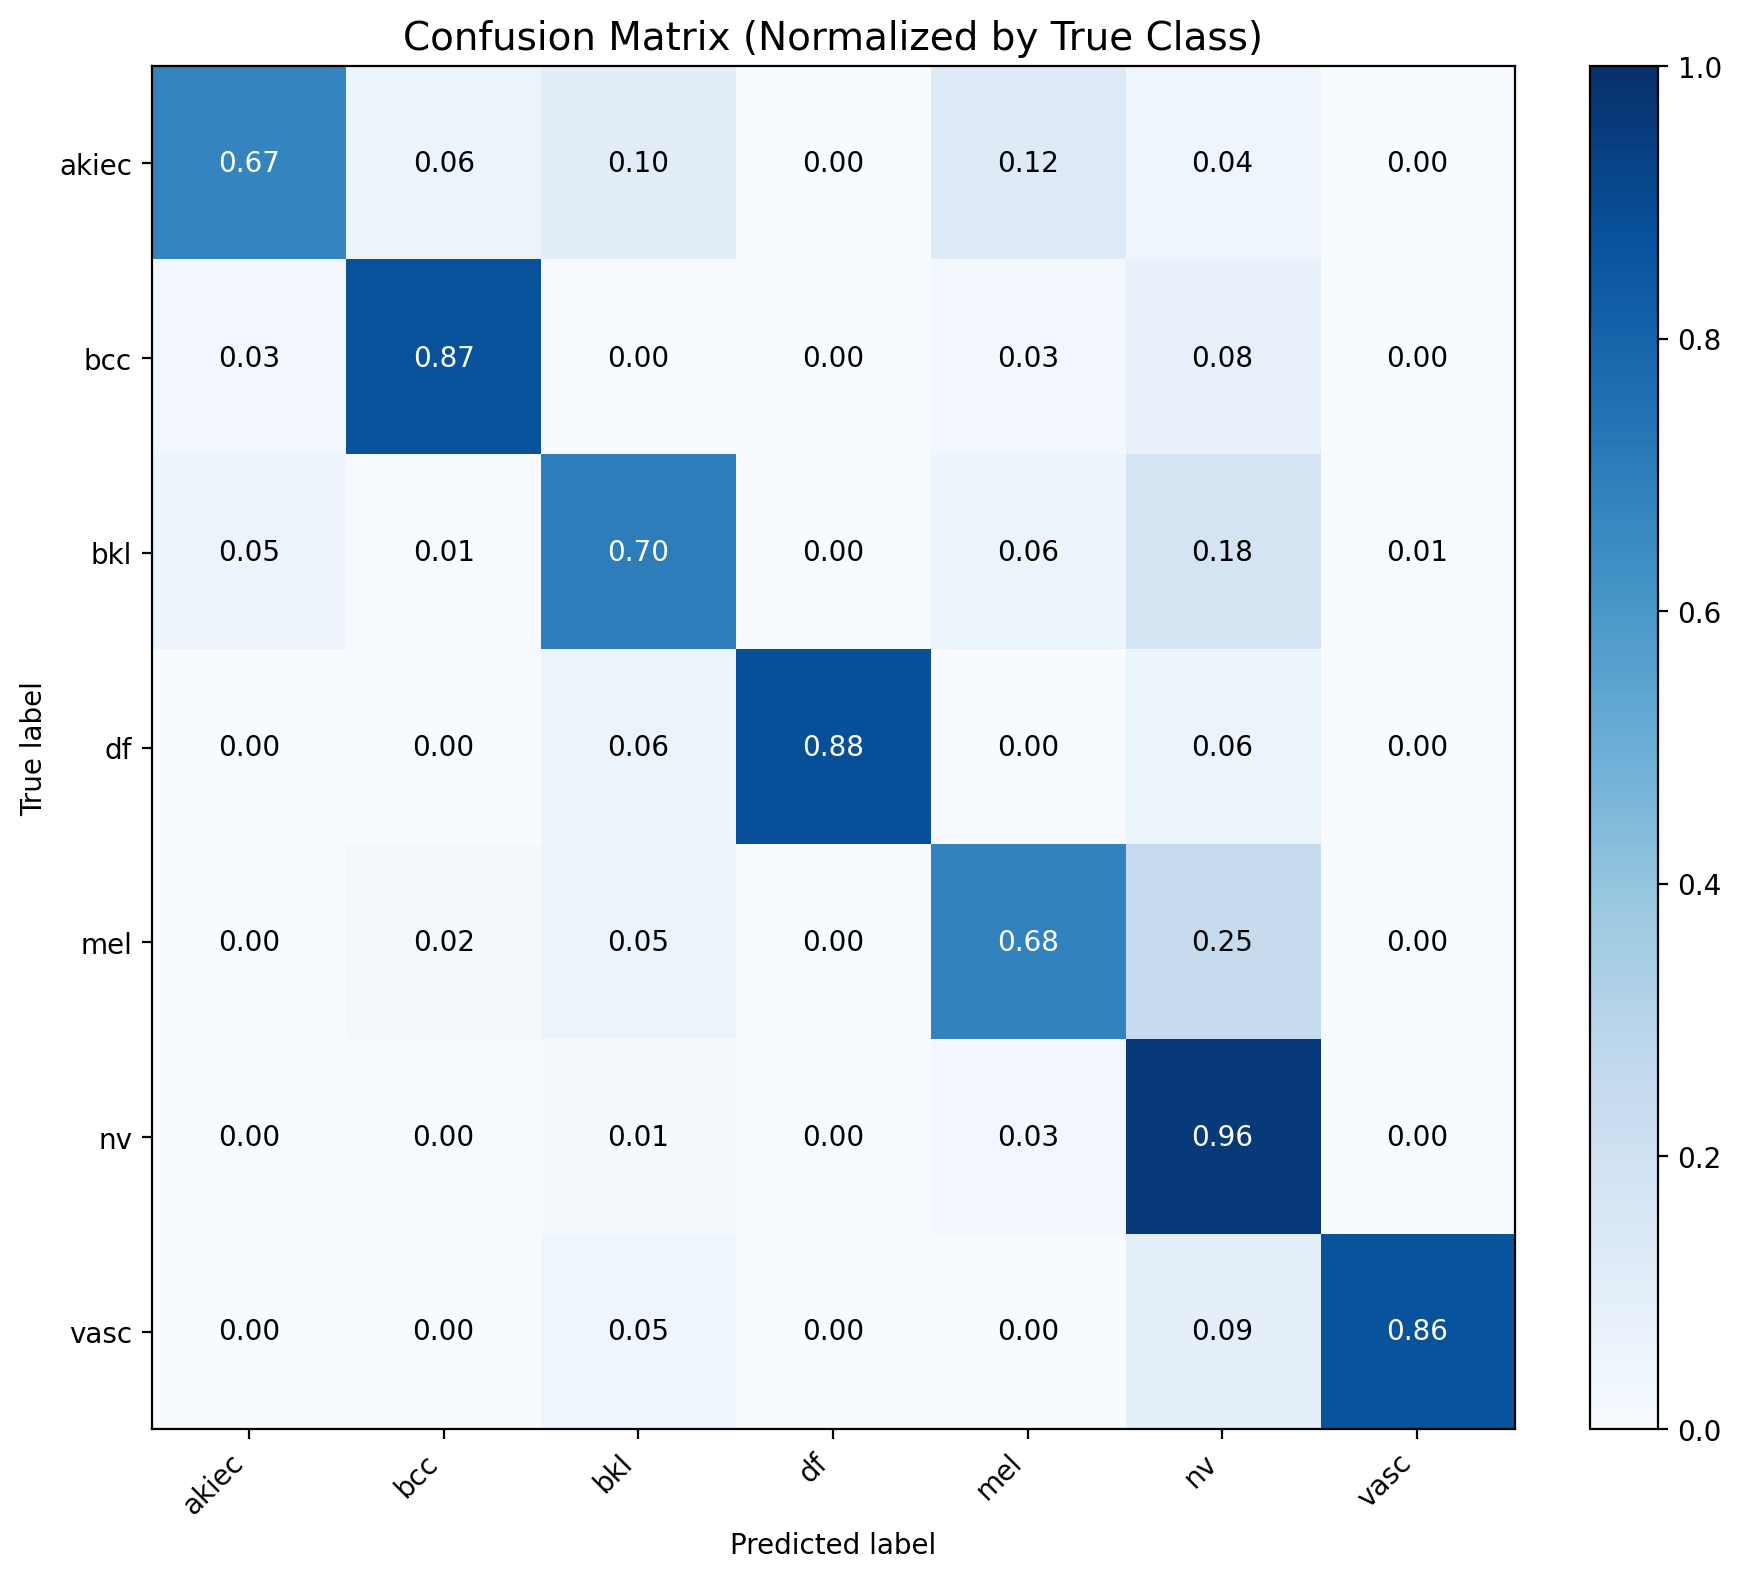
\includegraphics[width=\linewidth,height=3.4cm,keepaspectratio]{../thesis/figures/eb0_confusion_matrix.png}\\[4pt]
        \centering \textbf{DenseNet121}\\[2pt]
        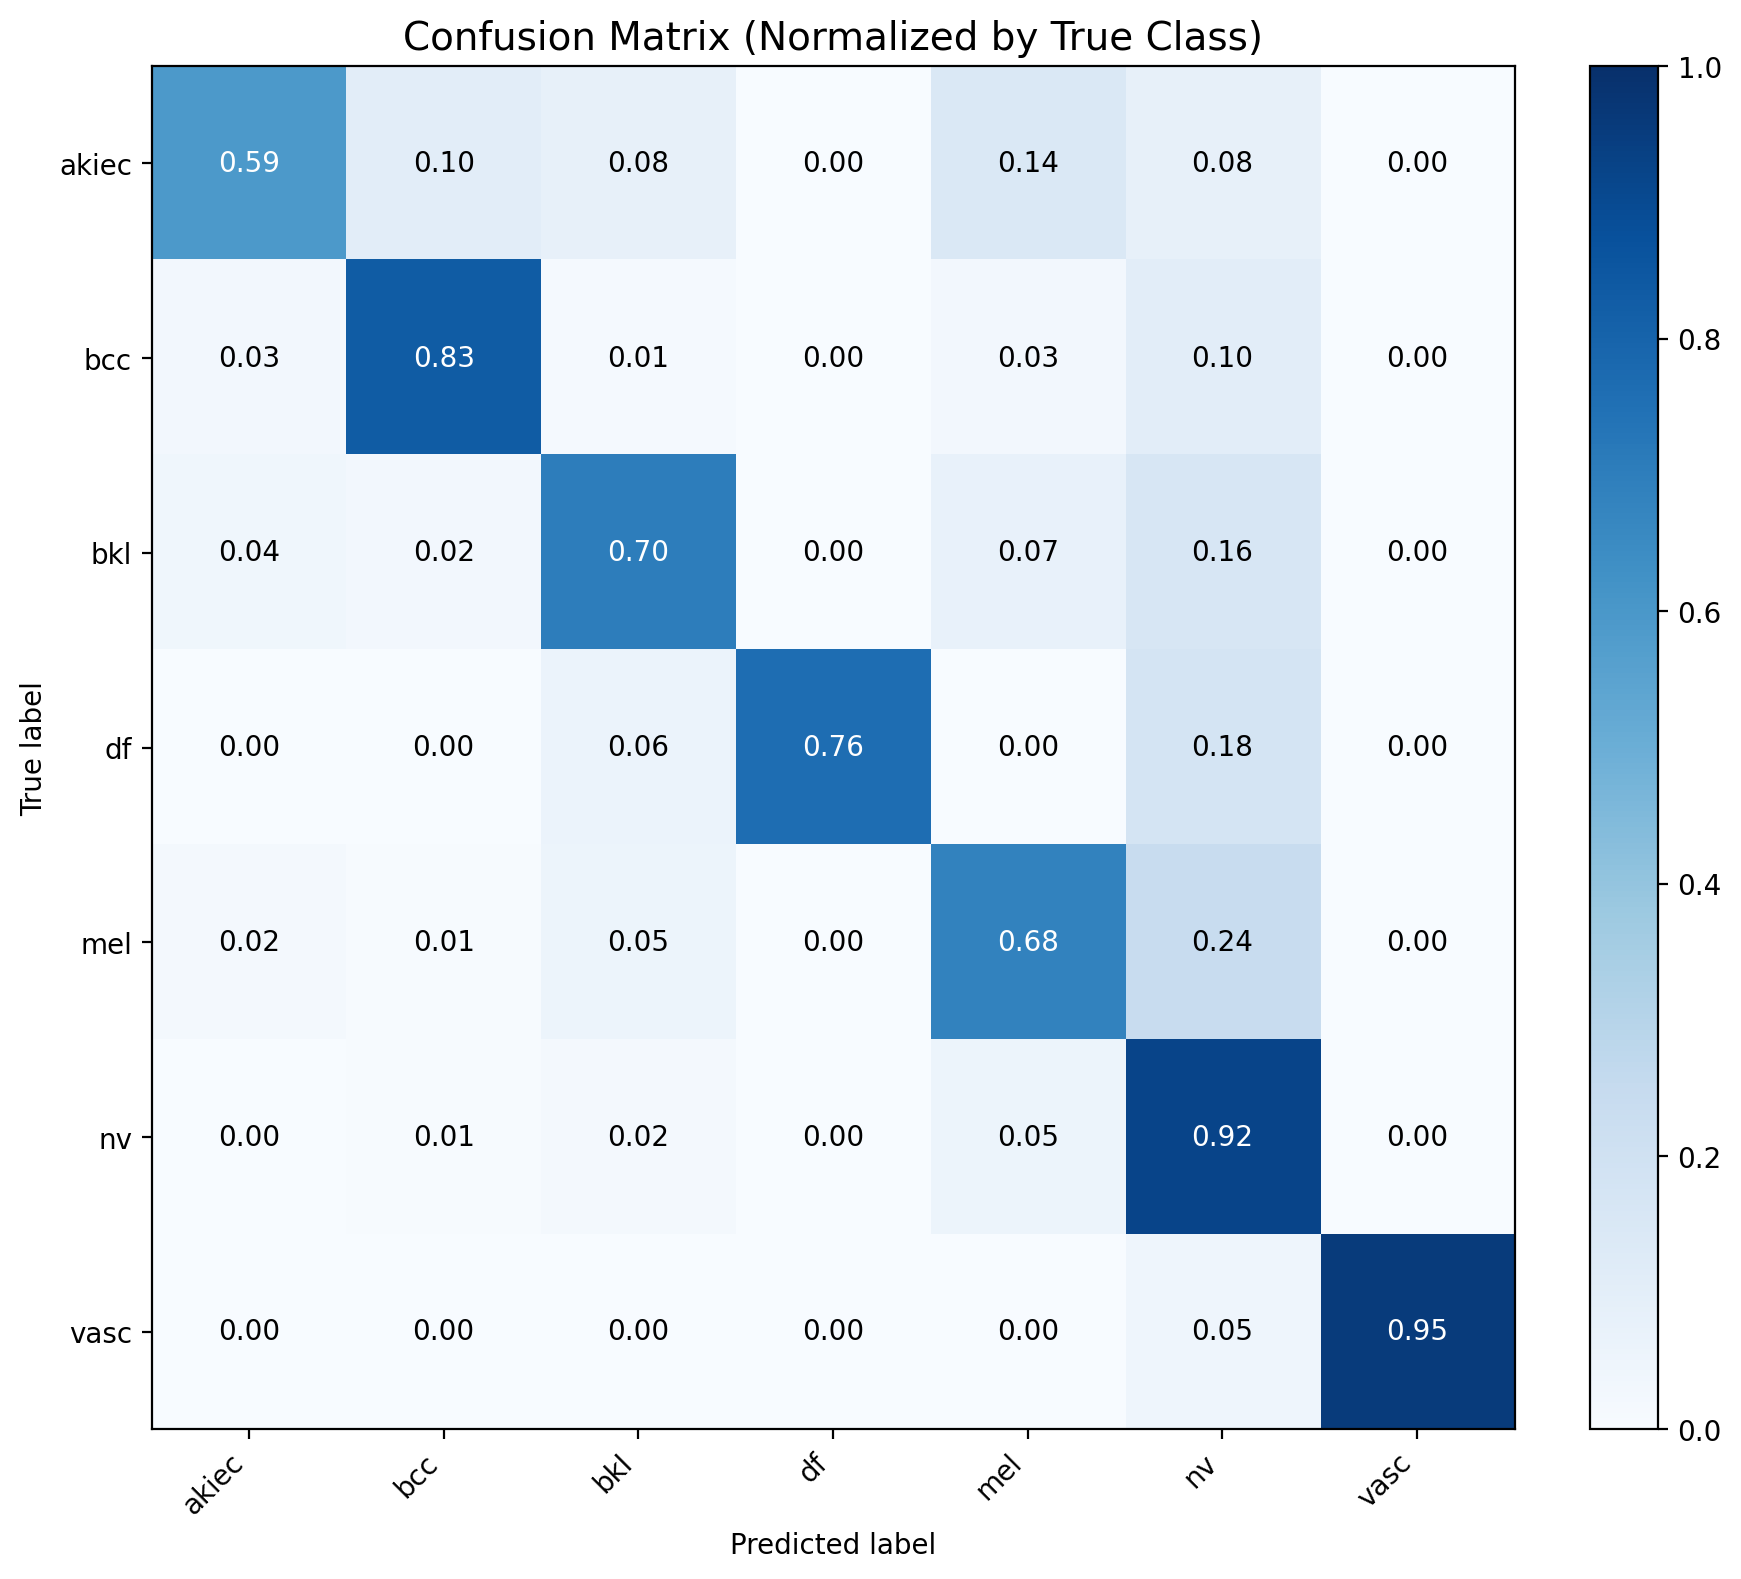
\includegraphics[width=\linewidth,height=3.4cm,keepaspectratio]{../thesis/figures/dn121_confusion_matrix.png}

        \column{0.5\textwidth}
        \centering \textbf{ResNet50}\\[2pt]
        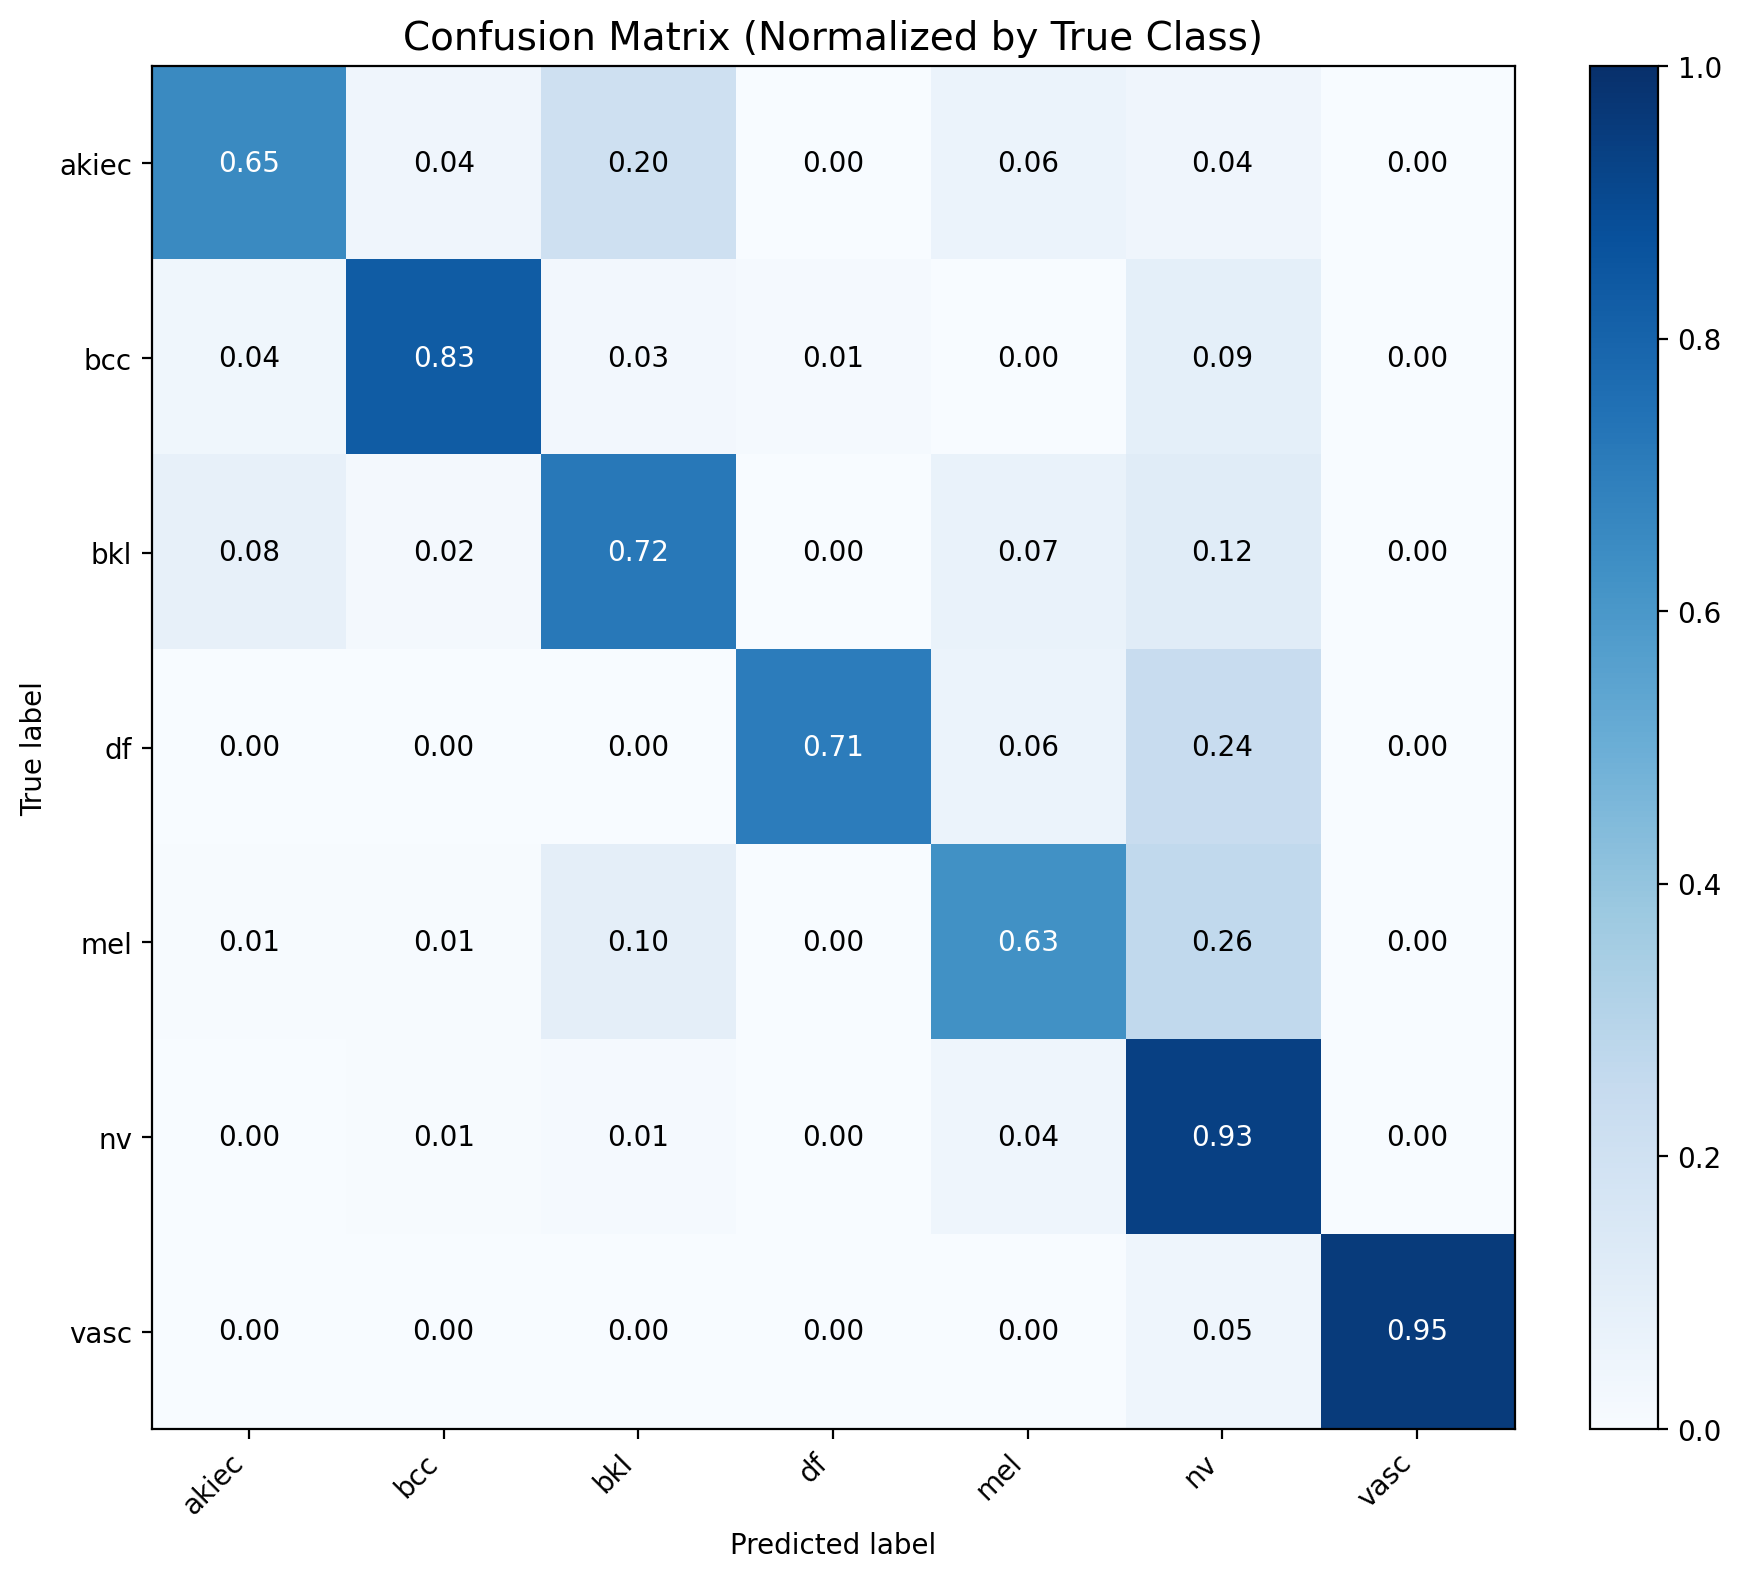
\includegraphics[width=\linewidth,height=3.4cm,keepaspectratio]{../thesis/figures/rn50_confusion_matrix.png}\\[4pt]
        \centering \textbf{Swin-Tiny}\\[2pt]
        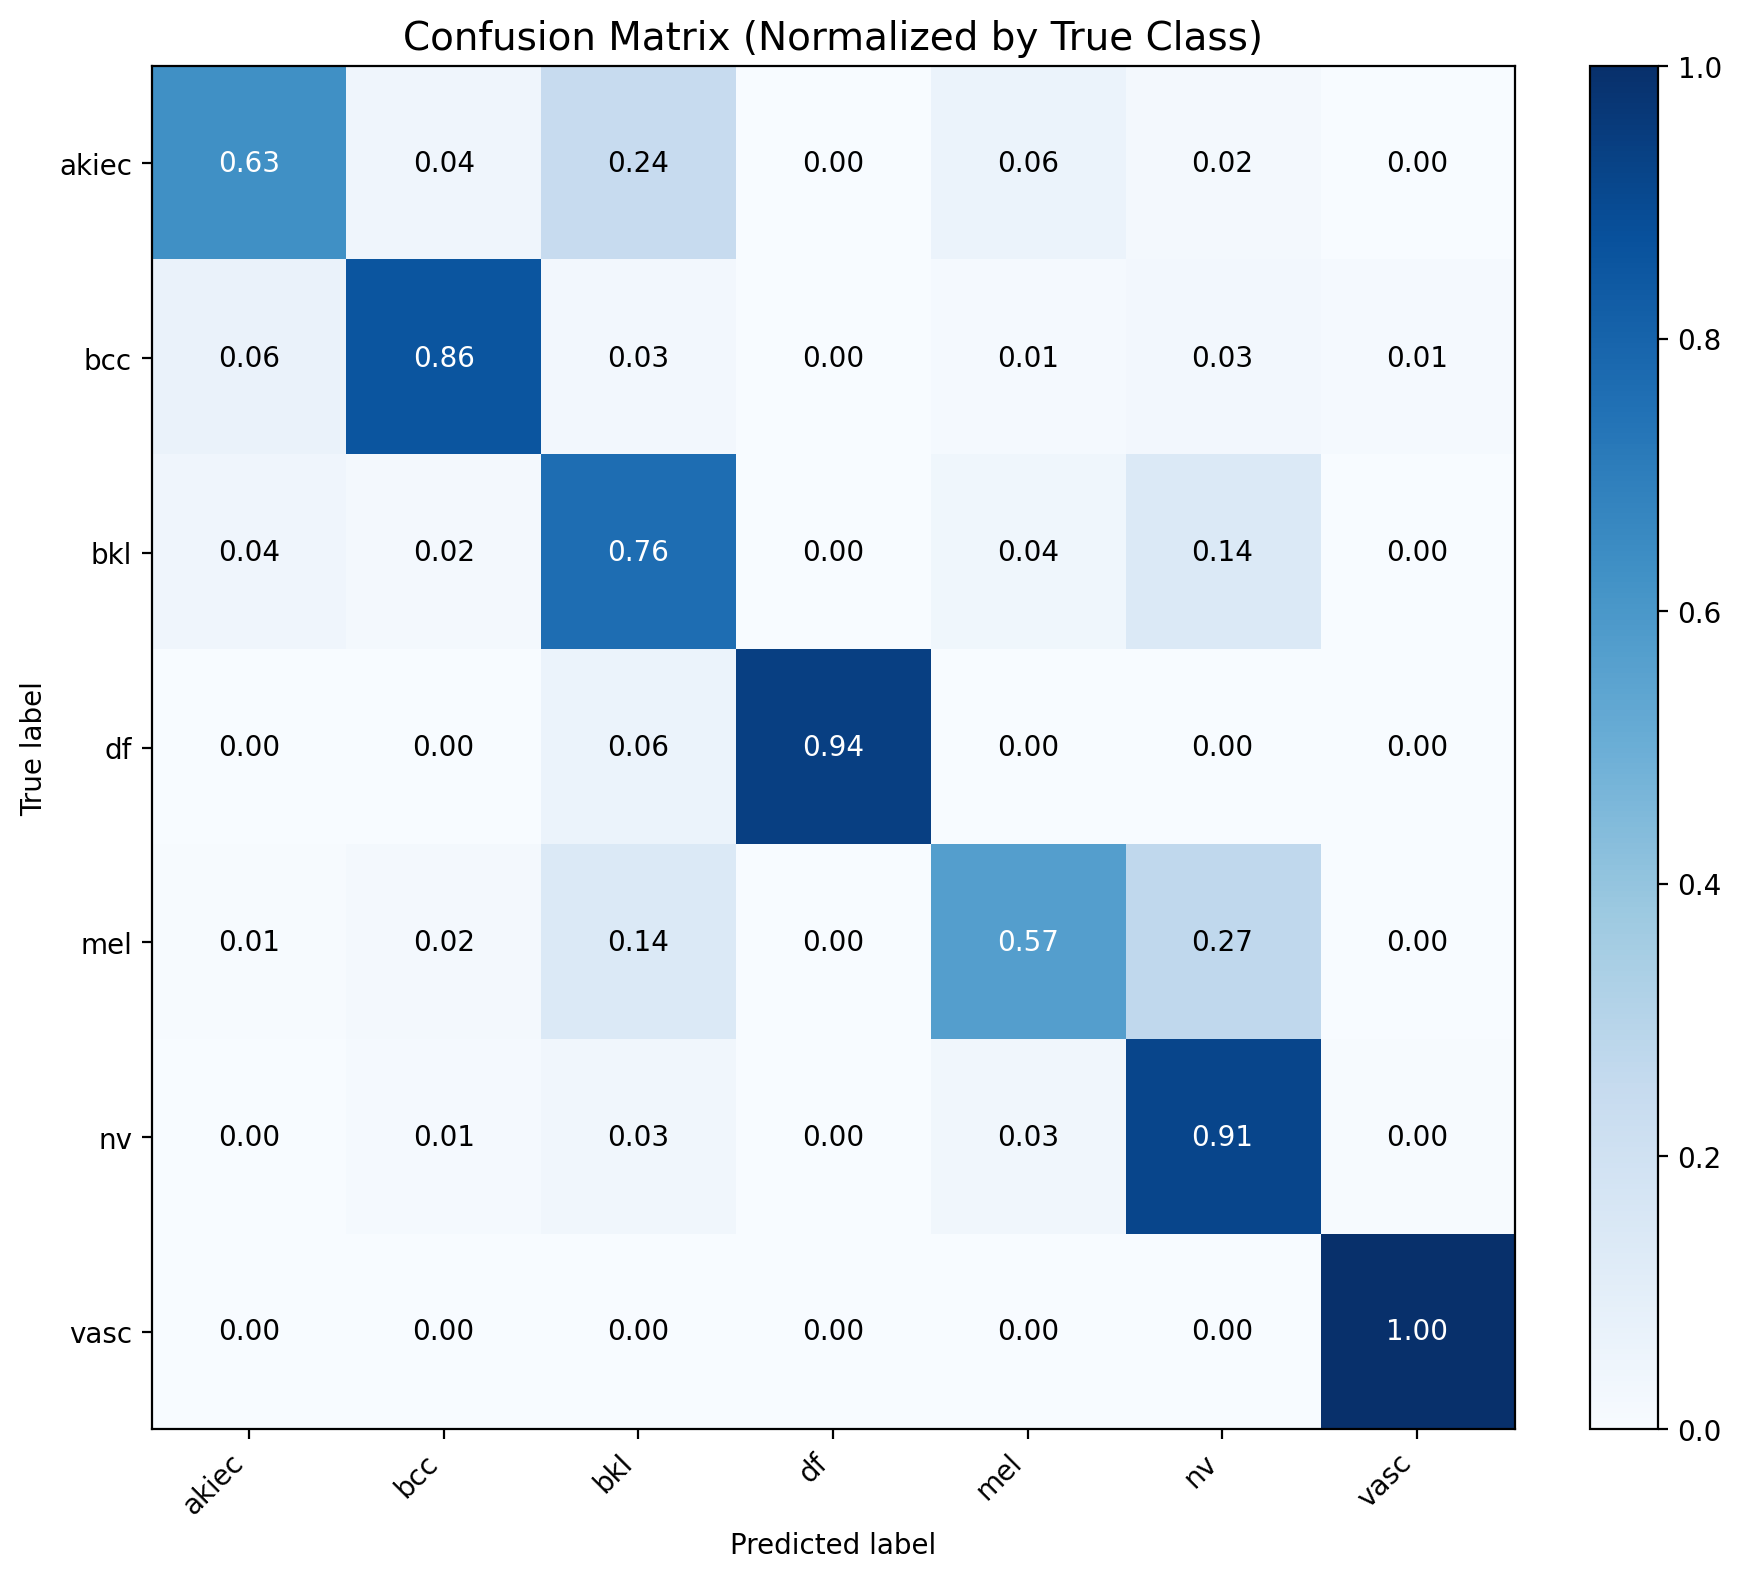
\includegraphics[width=\linewidth,height=3.4cm,keepaspectratio]{../thesis/figures/swin_confusion_matrix.png}
    \end{columns}
    \vspace{0.15cm}
    \scriptsize \textit{Every model shares the same failure mode --- confusion inside the \textbf{MEL $\leftrightarrow$ NV $\leftrightarrow$ BKL} cluster --- but each fails differently, which is exactly why the soft-voting ensemble improves over any single one.}
\end{frame}

% --- A27 ---
\begin{frame}{A27. Grad-CAM in Action --- From Image to Heatmap}
    \footnotesize
    \textit{Intuitive walkthrough. The rigorous formulas are in A7; the target layer per backbone is in A8.}
    \vspace{0.2cm}

    \begin{block}{Step 1 --- Forward pass}
        \scriptsize
        The image is pushed through the network. At the last convolutional block we tap the feature maps $A^k$: about $K=320$ (EB0) or $K=2048$ (RN50) channels, each a small $7 \times 7$ grid. Each channel encodes a different visual concept --- ``dark blob'', ``ring border'', ``streak''.
    \end{block}

    \begin{block}{Step 2 --- Backward pass through the predicted class}
        \scriptsize
        We call \texttt{loss.backward()} but only on the score of the predicted class $c$ (say, MEL). PyTorch fills the gradient $\partial y^c / \partial A^k$ --- ``if I nudged this channel up, would the MEL score go up too?''.
    \end{block}

    \begin{block}{Step 3 --- Channel importance $\alpha_c^k$}
        \scriptsize
        Average each channel's gradient over its $7 \times 7$ grid. A large positive $\alpha_c^k$ means channel $k$ pushes toward MEL; a negative one pushes away.
    \end{block}

    \begin{block}{Step 4 --- Weighted sum + ReLU + upsample}
        \scriptsize
        Multiply each channel by its $\alpha$ and add them up: $L_c = \mathrm{ReLU}(\sum_k \alpha_c^k A^k)$. ReLU discards the negative parts (only ``evidence for MEL'', never ``evidence against''). Upsample the resulting $7 \times 7$ heatmap back to $224 \times 224$, colour it with JET, blend over the original image.
    \end{block}

    \vspace{0.1cm}
    {\centering \scriptsize \textbf{One-line summary:} the heatmap answers ``\textit{which pixels, if brightened, would make the model more confident about the predicted class}''.\par}
\end{frame}

% =====================  Final slide  =====================
\begin{frame}[plain]
    \centering
    \vspace{2cm}
    {\Huge \textbf{\textcolor{usthblue}{Ready for your questions}}}\\[1cm]
    
\begin{tikzpicture}
        \draw[usthblue, line width=1.5pt] (0,0) -- (8,0);
    \end{tikzpicture}\\[1cm]
    \footnotesize \textit{Nguyen Trong Bach --- 23BI14057 --- USTH ICT 2026}
\end{frame}

\end{document}
